%% 
%% Copyright 2019-2020 Elsevier Ltd
%% 
%% This file is part of the 'CAS Bundle'.
%% --------------------------------------
%% 
%% It may be distributed under the conditions of the LaTeX Project Public
%% License, either version 1.2 of this license or (at your option) any
%% later version.  The latest version of this license is in
%%    http://www.latex-project.org/lppl.txt
%% and version 1.2 or later is part of all distributions of LaTeX
%% version 1999/12/01 or later.
%% 
%% The list of all files belonging to the 'CAS Bundle' is
%% given in the file `manifest.txt'.
%% 
%% Template article for cas-dc documentclass for 
%% double column output.

%\documentclass[a4paper,fleqn,longmktitle]{cas-dc}
\documentclass[a4paper,fleqn]{cas-dc}

%\usepackage[numbers]{natbib}
%\usepackage[authoryear]{natbib}
\usepackage[authoryear,longnamesfirst]{natbib}
\usepackage{graphicx} 
\usepackage{float}
\usepackage{amsmath}
\usepackage{caption}
\usepackage{listings}
\usepackage{xcolor}
\usepackage{listings}
\setcitestyle{numbers,square}



\usepackage[commandnameprefix=always]{changes}
\definecolor{blue}{RGB}{0, 100, 0}
\definecolor{blue}{RGB}{220, 20, 60}
\definecolor{blue}{RGB}{128, 0, 128}



\usepackage{pifont}       % \ding{xx}
\usepackage{bbding}       % \Checkmark,\XSolid,... (需要和pifont宏包共同使用)
\usepackage{fontawesome}  % \faCheck,\faTimes
 
% 采用如下宏定义更方便
\newcommand{\cmark}{\ding{51}}
\newcommand{\xmark}{\ding{55}}
\newcommand{\crossmark}{\ding{53}}

%%%Author definitions
\def\tsc#1{\csdef{#1}{\textsc{\lowercase{#1}}\xspace}}
\tsc{WGM}
\tsc{QE}
\tsc{EP}
\tsc{PMS}
\tsc{BEC}
\tsc{DE}
%%%

% Uncomment and use as needed
%\newtheorem{theorem}{Theorem}
%\newtheorem{lemma}[theorem]{Lemma}
%\newdefinition{rmk}{Remark}
%\newproof{pf}{Proof}
%\newproof{pot}{Proof of Theorem \ref{thm}}

\begin{document}
\let\WriteBookmarks\relax
\def\floatpagepagefraction{1}
\def\textpagefraction{.001}

% Short title
\shorttitle{WCANet: Effective Feature Modeling under Low Computational Cost}

% Short author
\shortauthors{Fang Wang et~al.}

% Main title of the paper
\title [mode = title]{WCANet: Effective Feature Modeling under Low Computational Cost}                      





\author[1]{Fang Wang}
\fnmark[1]

\affiliation[1]{organization={College of Information Engineering},
    addressline={Beijing Institute of Petrochemical Technology}, 
    city={Beijing},
    % citysep={}, % Uncomment if no comma needed between city and postcode
    postcode={102617}, 
    % state={},
    country={People's Republic of China}}



\author[1]{Huitao Li}



\author[2]{Wenhan Chao}

\affiliation[2]{organization={School of Computer Science and Engineering},
    addressline={Beihang University}, 
    city={Beijing},
    % citysep={}, % Uncomment if no comma needed between city and postcode
    postcode={100191,100083}, 
    % state={},
    country={People's Republic of China}}



\author[1]{Zheng Zhuo}[
orcid=0000-0001-8028-5285
]
\ead{zz@bipt.edu.cn}
\cormark[1]

\author[1]{Xinxin Yang}



\cortext[cor1]{Corresponding author}

% Here goes the abstract
\begin{abstract}
To design efficient neural networks, many studies focus on reducing redundancy. However, such feature discarding is often random and may remove useful information, which leads to degraded network performance. To address the challenge of insufficient feature extraction under limited computational budgets, we decouple feature modeling into channel-wise and spatial dimensions, which substantially reduces computational overhead. To enable efficient spatial modeling, we propose Learnable Wavelet Spatial Attention (LWSA), which leverages the wavelet transform to decompose the feature map into multiple subbands of varying informativeness and performs spatial attention selectively on the most informative components, enabling effective feature extraction at low computational cost. By cascading the ESE module and LWSA, we propose a Cascaded Channel–Spatial Attention mechanism for feature extraction. Building upon this, we further introduce WCANet, a lightweight architecture that achieves effective feature modeling under low computational budgets across a variety of vision tasks. For example, on the ImageNet-1K, WCANet significantly outperforms FasterNet in accuracy while achieving 40\% higher throughput. WCANet-T4 runs 2.9× faster than StarNet-S1 with 1.4\% higher accuracy, and also surpasses MobileMamba-T2 by 1.3\% in Top-1 accuracy while maintaining high efficiency. 

\end{abstract}

% Use if a graphical abstract is present
% \begin{graphicalabstract}
% \includegraphics{grabs.pdf}
% \end{graphicalabstract}


\begin{graphicalabstract}
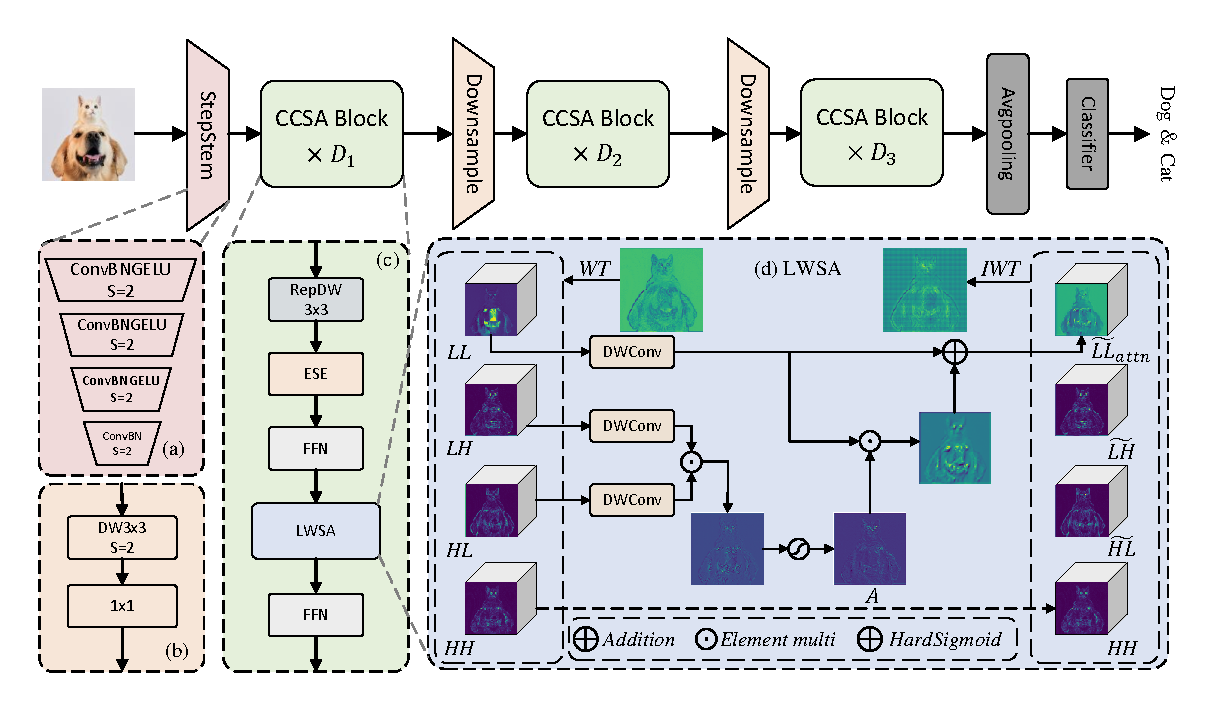
\includegraphics[width=1\linewidth]{WCANet.pdf}


To design efficient neural networks, many studies focus on reducing redundancy. However, such feature discarding is often random and may remove useful information, which leads to degraded network performance. To address the challenge of insufficient feature extraction under limited computational budgets, we decouple feature modeling into channel-wise and spatial dimensions, which substantially reduces computational overhead. To enable efficient spatial modeling, we propose Learnable Wavelet Spatial Attention (LWSA), which leverages the wavelet transform to decompose the feature map into multiple subbands of varying informativeness and performs spatial attention selectively on the most informative components, enabling effective feature extraction at low computational cost. By cascading the ESE module and LWSA, we propose a Cascaded Channel–Spatial Attention mechanism for feature extraction. Building upon this, we further introduce WCANet, a lightweight architecture that achieves effective feature modeling under low computational budgets across a variety of vision tasks. For example, on the ImageNet-1K, WCANet significantly outperforms FasterNet in accuracy while achieving 40\% higher throughput. WCANet-T4 runs 2.9× faster than StarNet-S1 with 1.4\% higher accuracy, and also surpasses MobileMamba-T2 by 1.3\% in Top-1 accuracy while maintaining high efficiency. 

\end{graphicalabstract}

% Research highlights
\begin{highlights}
{ \color{blue}
 \item {To overcome the limitation that fixed wavelet filters cannot effectively decompose high-dimensional feature maps, we propose learnable wavelet filters with orthogonality constraints, allowing filters to adapt dynamically while strictly maintaining orthogonality.}
  
  \item {We propose a learnable wavelet spatial attention mechanism (LWSA). LWSA leverages the features from sub-bands with different orientations to perform spatial attention on informative sub-bands, thereby enhancing key spatial nodes and achieving efficient spatial feature modeling.}

  \item {We propose Cascade Channel–Spatial Attention (CCSA). CCSA utilizes ESE and LWSA to perceive key features at both channel and spatial levels, respectively, achieving an optimized accuracy-efficiency trade-off.}

 \item {We propose WCANet, a visual network design optimized for practical lightweight applications. Extensive experiments demonstrate that WCANet exhibits robust scalability and highly competitive performance across various devices.}

 }
\end{highlights}

% Keywords
% Each keyword is separated by \sep
\begin{keywords}
Vision Transformer \sep Image Classification \sep Object Detection \sep 
\end{keywords}


\maketitle



\section{Introduction}

With the proliferation of mobile devices, lightweight network designs have become a research hotspot in vision network design~\cite{han2022survey,he2016deep,dosovitskiy2020image,liu2022convnet,liu2021swin,zhang2024vision}. Current mainstream lightweight models are primarily categorized into CNN-based, Transformer-based, and Mamba-based structures. Vision Transformers (ViTs) have drawn significant attention due to their global effective receptive field (ERF) and strong long-range dependency modeling capability. However, their quadratic computational complexity leads to substantially higher inference overhead compared to other architectures. Although {\color{blue} some works~\cite{li2022efficientformer,maaz2022edgenext,liu2023efficientvit,mehta2021mobilevit,wadekar2022mobilevitv3,yun2024shvit,khan2025optimal}} have been proposed to alleviate this issue with notable success, the computational bottleneck of ViTs still becomes evident under high-resolution inputs.

State-space models (SSMs)~\cite{fu2022hungry,gu2024mamba,gu2021efficiently,smith2022simplified} are able to capture long-range dependencies with linear computational complexity, motivating researchers to explore their application in vision tasks. Consequently, SSMs have been successfully adapted to the visual domain and have achieved notable results~\cite{liu2024vmamba,pei2025efficientvmamba}. MobileMamba~\cite{he2025mobilemamba}, as a lightweight Mamba-based architecture, has achieved high throughput and high precision on the GPU. However, vision mambas (ViMs) are limited by GPU device support, and the inference latency on devices such as CPU will increase significantly. This severely restricts the performance of these methods in practical applications.

CNN-based methods~\cite{sandler2018mobilenetv2,wadekar2022mobilevitv3,tan2021efficientnetv2} aim to achieve model lightweighting by reducing \chreplaced{\color{blue}computational overhead}{\color{blue}redundancy}. Early works~\cite{howard2017mobilenets,tan2019rethinking,ma2018shufflenet,zhang2018shufflenet} leveraged DWConv to lower computational redundancy but overlooked actual runtime efficiency. Some methods \cite{han2020ghostnet,tang2022ghostnetv2} like FasterNet~\cite{chen2023run} improve the computational efficiency by reducing the extraction of redundant features. However, existing methods \cite{han2020ghostnet,chen2023run} \chreplaced{\color{blue}often struggle to balance representational capacity and computational efficiency in lightweight CNN design}{\color{blue} have not truly achieved the separation of effective features and redundant features}. \chreplaced{\color{blue} Aggressively discarding spatial details can lead to the loss of potentially useful information}{\color{blue} Many potentially useful features in the unutilized parts have not been extracted}, thereby limiting the model's feature representation ability. Coupled with the limited receptive field of convolution, this has caused CNNs to lag \chdeleted{\color{blue}significantly }in accuracy compared to other architectures. To break through the performance bottleneck of CNN-based methods, this paper proposes a new \chreplaced{\color{blue}lightweight feature modeling paradigm}{\color{blue}feature separation method and a new feature extraction method}.

\begin{figure}
    \centering
    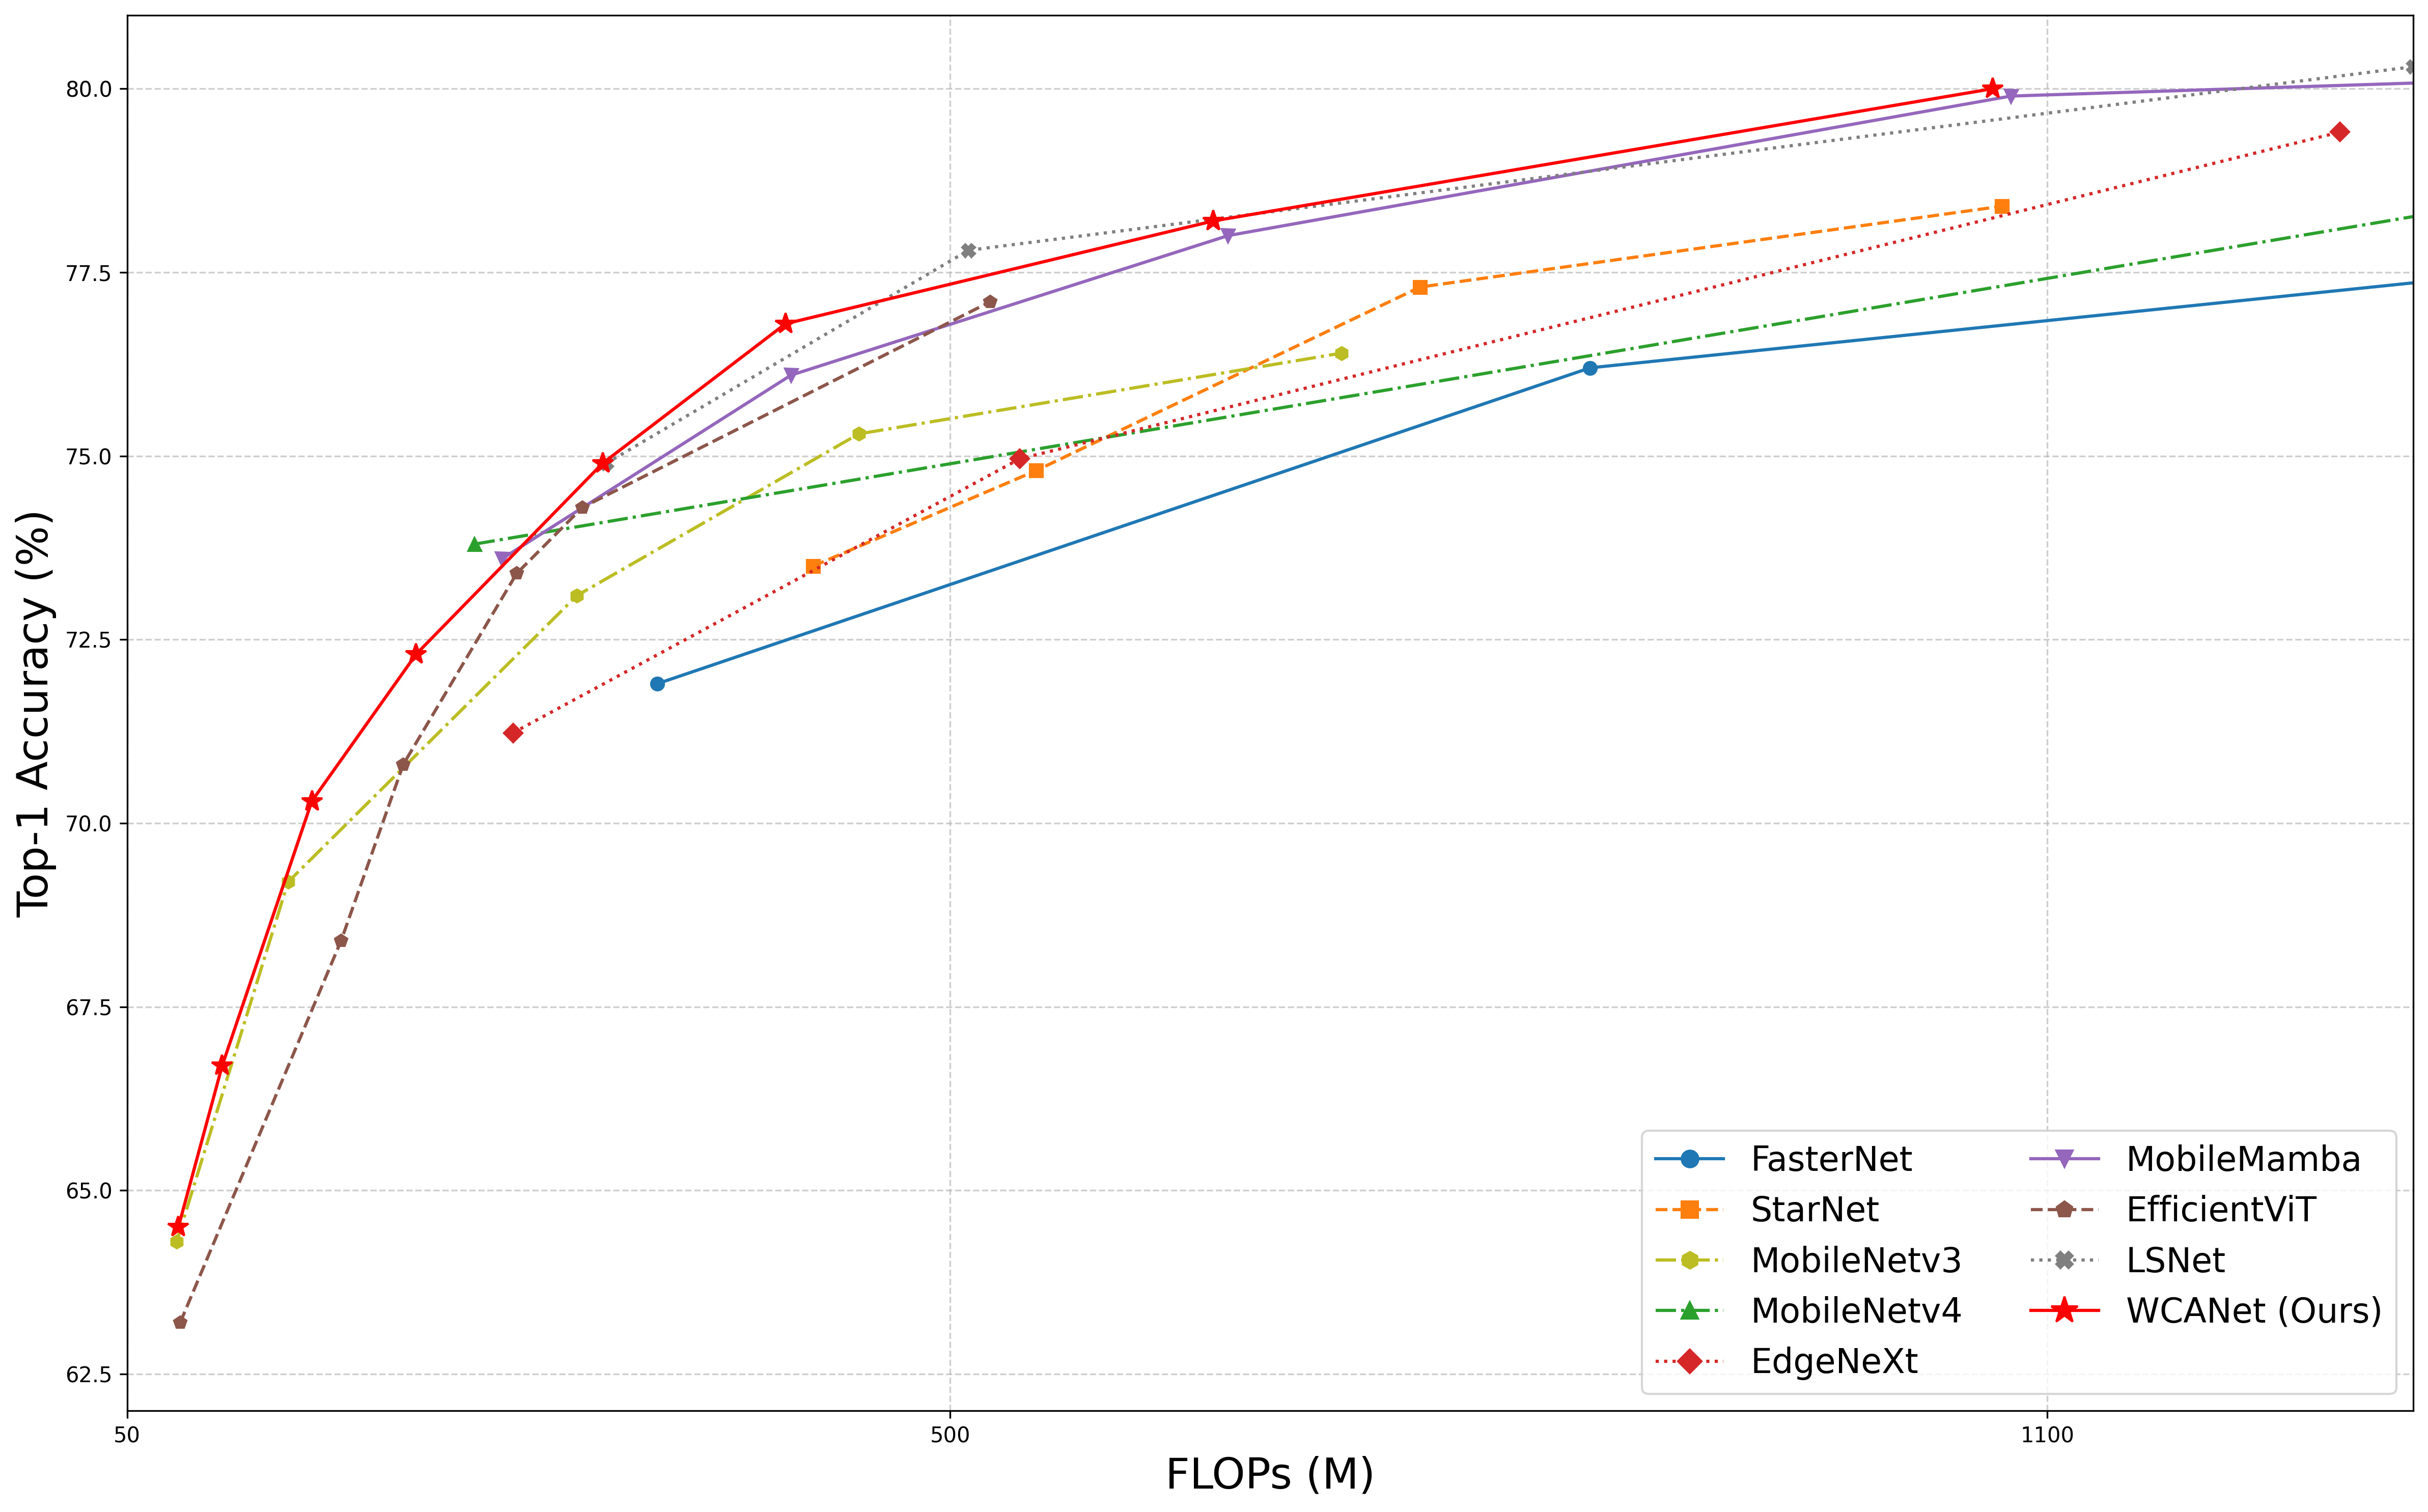
\includegraphics[width=1.\linewidth]{flops_vs_top1_linear_custom_ticks_new.png}
    \caption{Performance vs. FLOPs with SoTA methods}
    \label{fig:vs_acc}
\end{figure}

To achieve \chreplaced{\color{blue} highly efficient spatial feature extraction}{\color{blue} effective separation of redundant features}, this paper introduces the wavelet transform~\cite{daubechies1992ten}. We decompose the input feature map into four sub-bands, based on the differences in the information contained in each sub-band. As shown in Fig.\ref{fig:ll_lh_hl_hh}, the LL, LH, and HL sub-bands possess more abundant features. Therefore, we regard them as \chreplaced{\color{blue} informative}{effective} feature sub-bands. However, the HH sub-band only contains a small amount of high-frequency \chreplaced{\color{blue} noise or sparse details}{features}. Considering operational efficiency, we do not perform feature extraction on the HH sub-band\chadded{ \color{blue}, thereby strictly bounding the computational overhead}.

Based on the above \chreplaced{\color{blue} frequency-aware principles}{feature separation methods}, this paper proposes the Cascade Channel–Spatial Attention (CCSA) module. CCSA decouples feature modeling into channel-wise and spatial levels. Firstly, CCSA uses the Effective Squeeze and Extraction (ESE) module~\cite{lee2020centermask} to enhance the responses of key channels; subsequently, we {\color{blue}introduce} the Learnable Wavelet Spatial Attention (LWSA) to achieve \chreplaced{\color{blue} hardware-friendly lightweight CNN design and efficient spatial modeling}{the separation of redundant features in the spatial level and effective spatial modeling}. LWSA uses the wavelet transform to separate the \chdeleted{redundant }HH sub-band. Then, based on the complementary characteristics of the LH and HL sub-bands, LWSA generates a spatial attention weight map, which is applied to the LL sub-band with the richest semantic information to enhance the important spatial regions. Finally, the feature map is restored to its original size through inverse wavelet transform.

Based on CCSA, this paper proposes WCANet (Wavelet Cascade Attention Network), a lightweight vision network for resource-constrained scenarios. WCANet \chreplaced{\color{blue} achieves an optimal balance between accuracy and inference latency, providing a highly effective lightweight CNN design}{truly achieves the separation of effective features and redundant features, completing efficient feature modeling with extremely low computational cost}. Fig.\ref{fig:vs_acc} and Fig.\ref{fig:GPU_throught} show that WCANet \chreplaced{ \color{blue} demonstrates highly competitive performance against}{surpasses} existing SoTA methods. \chadded{Specifically, WCANet maintains a consistent performance upper hand across the entire evaluation spectrum (from 80M to 1078M FLOPs). }  Experiments show that WCANet is \chreplaced{highly effective for}{suitable for extremely} lightweight scenarios: on ImageNet-1K, WCANet-T1 achieves a Top-1 accuracy of 64.5\% with only 80M FLOPs, surpassing EfficientViT-M0 by 1.3\%. In lightweight application scenarios with more relaxed computational resources, WCANet also \chreplaced{\color{blue} exhibits strong scalability}{performs extremely well}: the Top-1 accuracy of WCANet-T4, T6, and T8 is 3\%, 2\%, and 1.1\% higher than that of FasterNet-T0, T1, and T2, respectively, while the throughput is increased by an average of 40\%. Under the same throughput\chadded{,} WCANet achieves a \chreplaced{\color{blue} performance}{throughput} comparable to MobileMamba while surpassing it in Top-1 accuracy across the board, and has a significantly lower inference latency on CPUs than MobileMamba. 

To summarize, our contributions are as follows:

% \begin{itemize}
%   \item We propose learnable wavelet filters with orthogonality constraints to improve the adaptability of wavelet transforms to high-dimensional features.
  
%   \item We propose a learnable wavelet spatial attention mechanism. LWSA performs spatial attention operations on \chreplaced{\color{blue} informative}{effective} feature sub-bands to enhance key spatial nodes, achieving \chreplaced{ \color{blue} hardware-efficient}{effective} spatial feature modeling.

%   \item We propose Cascade Channel–Spatial Attention (CCSA). CCSA utilizes ESE and LWSA to respectively perceive the key features in the channel-wise and the spatial level, achieving \chreplaced{\color{blue} an optimized accuracy-efficiency trade-off}{efficient extraction of effective features under low computational cost}.

%  \item We propose WCANet, a lightweight visual network design \chreplaced{\color{blue} optimized for}{for practical} lightweight applications. Extensive experiments show that WCANet \chreplaced{\color{blue} demonstrates robust scalability and highly competitive}{has powerful and efficient} performance on both GPU and CPU devices.
% \end{itemize}

\begin{itemize}

{ \color{blue}
 \item {To overcome the limitation that fixed wavelet filters cannot effectively decompose high-dimensional feature maps, we propose learnable wavelet filters with orthogonality constraints, allowing filters to adapt dynamically while strictly maintaining orthogonality.}
  
  \item {We propose a learnable wavelet spatial attention mechanism (LWSA). LWSA leverages the features from sub-bands with different orientations to perform spatial attention on informative sub-bands, thereby enhancing key spatial nodes and achieving efficient spatial feature modeling.}

  \item {We propose Cascade Channel–Spatial Attention (CCSA). CCSA utilizes ESE and LWSA to perceive key features at both channel and spatial levels, respectively, achieving an optimized accuracy-efficiency trade-off.}

 \item {We propose WCANet, a visual network design optimized for practical lightweight applications. Extensive experiments demonstrate that WCANet exhibits robust scalability and highly competitive performance across various devices.}

 }
\end{itemize}






\begin{figure}[width=1\linewidth,pos=t]
    \centering
    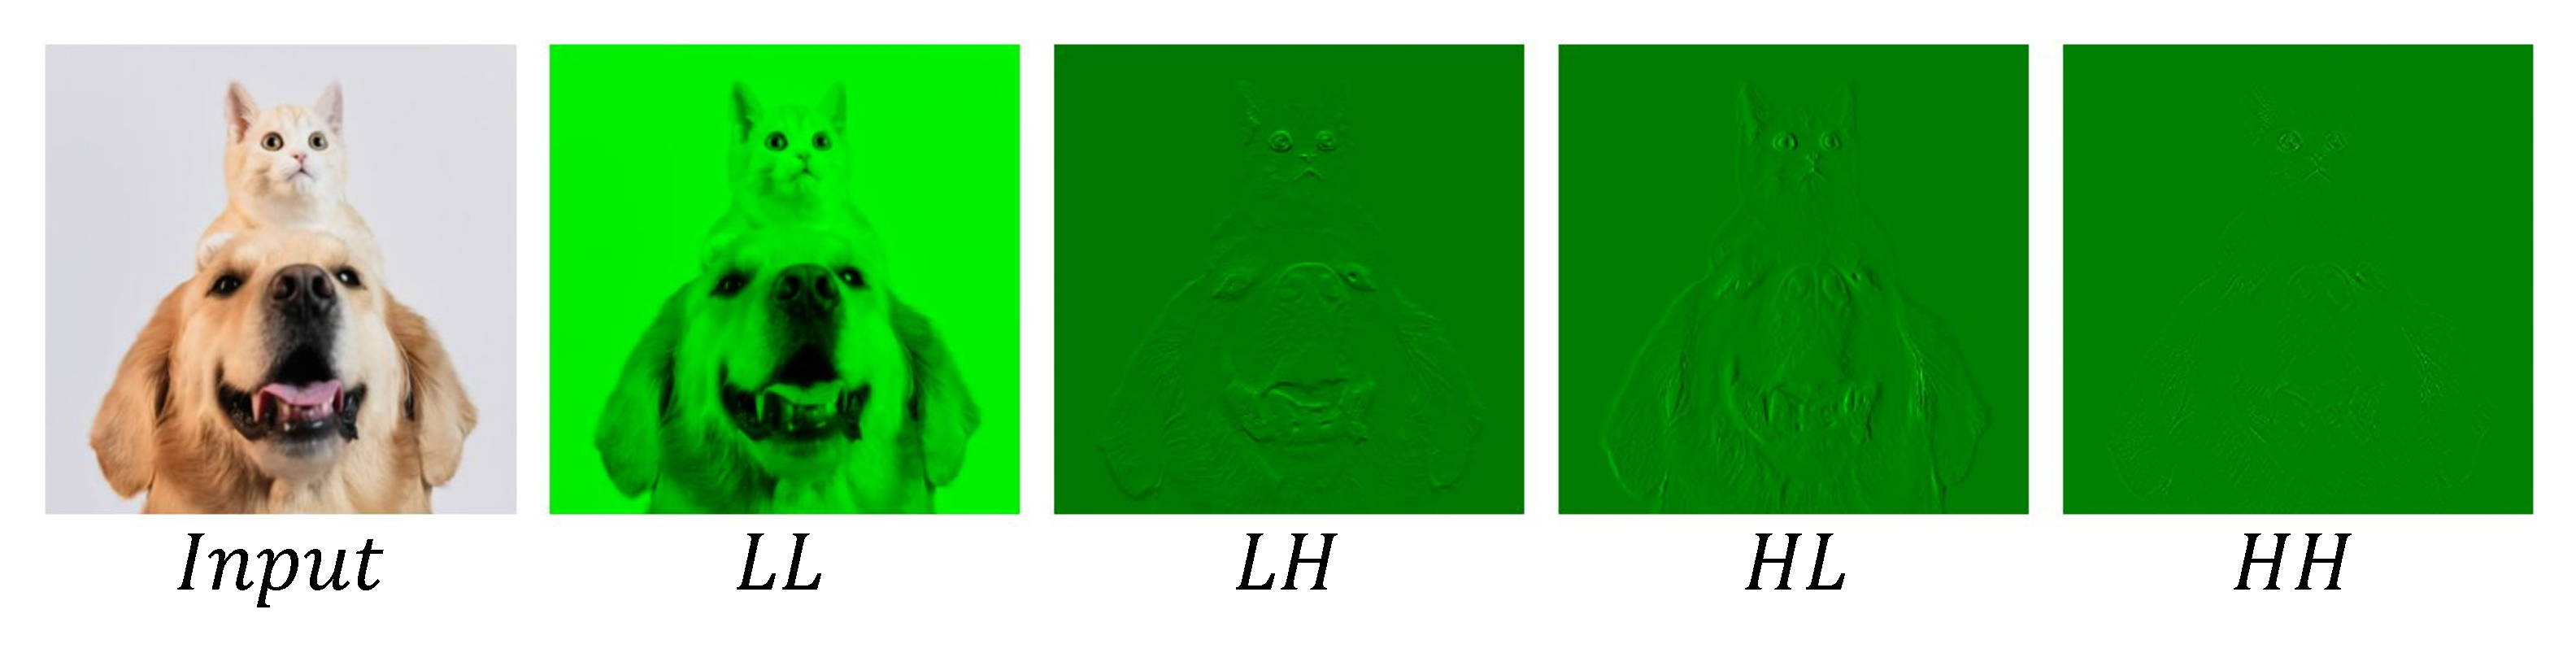
\includegraphics[width=1\linewidth]{LL_LH_HL_HH.pdf}
    \caption{Wavelet decomposition sub-bands. The four sub-bands (LL, LH, HL, HH) are obtained by applying the learnable wavelet transform to an input image.}
    \label{fig:ll_lh_hl_hh}
\end{figure}


























\section{Related Work}


\subsection{Lightweight network design}

\textbf{ViT-based methods.} Since the Transformer \cite{vaswani2017attention} was introduced to computer vision \cite{dosovitskiy2020image}, various networks based on the Transformer architecture have demonstrated powerful capabilities in various computer vision tasks \cite{esser2021taming, zhang2022topformer, liu2021swin}. Some works have attempted to combine the ideas of ViT and CNN for application in lightweight tasks \cite{li2022efficientformer, mehta2022separable, vasu2023fastvit, wang2025cait}. For instance, MobileViT \cite{mehta2021mobilevit} integrates MHSA with MobileNets to achieve an architectural hybrid. EdgeViT \cite{pan2022edgevits} proposes the integration of self-attention and convolutions to achieve cost-effective information exchange. In addition, to enhance the actual operational efficiency, MobileViTv2 \cite{mehta2022separable} proposes a linear complexity Transformer architecture to reduce the inference cost. FastViT \cite{vasu2023fastvit} introduces structural re-parameterization to increase the running speed. SHViT\cite{yun2024shvit} proposes single-head self-attention (SHSA), which improves the operational efficiency by performing attention calculations only on a portion of the channels.


% State Space Models (SSMs)
% Vision Mamba(Vim)采用双向 Mamba 块建模空间特征。Vmamba引入交叉扫描机制增强空间建模能力。
% EfficientVMamba使用skip sampling提高运行效率。

\textbf{SSM-based methods.} State Space Models (SSMs) \cite{fu2022hungry, gu2021efficiently, smith2022simplified} have attracted considerable interest because of their computational efficiency in modeling long-range dependencies. Mamba \cite{gu2024mamba} incorporates the S6 module, delivering a straightforward architecture that excels in efficiently modeling long sequences. Due to this advantage, many works have applied it to computer vision \cite{hatamizadeh2407mambavision, he2024mambaad, liu2024vmamba, zhu2024vision}. Vision Mamba (Vim) \cite{zhu2024vision} adopts bidirectional Mamba block modeling for spatial feature representation. Vmamba \cite{liu2024vmamba} introduces a  Cross-Scan mechanism to enhance spatial modeling capabilities. EfficientVMamba \cite{pei2025efficientvmamba}  improves efficiency by using skip sampling. MobileMamba \cite{he2025mobilemamba} designs a three-stage lightweight architecture with multi-receptive field interaction for high throughput.



\textbf{CNN-based methods.} Since AlexNet \cite{krizhevsky2012imagenet}, CNNs have been widely applied to various computer vision tasks \cite{redmon2016you,long2015fully,bolya2019yolact,dong2015image,wang2023hierarchical,ding2023exploring}. DWConv \cite{chollet2017xception} has greatly promoted the lightweight development of CNN. MobileNets \cite{howard2017mobilenets, sandler2018mobilenetv2, wadekar2022mobilevitv3}, ShuffleNets \cite{zhang2018shufflenet,ma2018shufflenet}, and EfficientNet \cite{tan2019rethinking} reduce computational redundancy by introducing DWConv and combine ingenious network structure designs to achieve powerful feature extraction capabilities at low computational costs. GhostNet \cite{han2020ghostnet} further observes that there is a high degree of redundancy among the channels of feature maps. By performing cheap linear operations only on some channels, it achieves efficient feature extraction capabilities. FasterNet \cite{chen2023run} achieves a significant improvement in operational efficiency by using PConv instead of DWConv.


\subsection{Wavelet Transforms in Deep Learning}

Wavelet transform~\cite{daubechies1992ten} was introduced to enhance the performance of the model in aspects such as multi-scale feature extraction, computational efficiency, or generation quality. The wavelet transform is used as the pooling operator in convolutional networks~\cite{duan2017sar,williams2018wavelet}. The wavelet transform is also employed to compress feature maps to reduce the computational cost of CNNs~\cite{finder2022wavelet}. In terms of network architecture design, some researchers have utilized wavelets for downsampling in the U-Net framework~\cite{ronneberger2015u} and implemented upsampling through inverse wavelet transform~\cite{liu2018multi,alaba2022wcnn3d}. The WTConv~\cite{finder2024wavelet} combines wavelet decomposition with convolution operations, effectively expanding the receptive field and enhancing the response to low-frequency structures.
\chadded{ \color{blue}However, while wavelet transforms have been successfully integrated into CNNs, current approaches typically process both high-frequency and low-frequency sub-bands equally without distinguishing their semantic richness. Further exploration is still needed to leverage the complementary characteristics of these sub-bands for dynamic feature modulation, especially under strictly limited computational budgets.}




















\section{Method}


\label{sec:intro}


\subsection{Revisiting Convolutions}


The process of the standard convolution operation is as follows:
given the input feature map $ X\in\mathbb{R}^{C\times H\times W} $ and the Standard Kernel $K\in\mathbb{R}^{ C_{out} \times C_{in}\times H\times W}$, the output feature map  $Y\in\mathbb{R}^{C_{out}\times H\times W}$ is:
\begin{equation}
   \centering 
    Y = X * K ,
\end{equation}
Specifically, $y_{[c',i,j]}$ is an element in the location $(i,j)$ at channel $c'$ of $Y$. The value of $y_{[c',i,j]}$ is calculated by:
\begin{equation}
   \centering 
        y_{\left\lbrack c^{\prime},i,j\right\rbrack}=\sum\limits_{c=1}^{C_{_{}in}}\sum\limits_{m=1}^{K}\sum\limits_{n=1}^{K}x_{\left\lbrack c,i+m,j+n\right\rbrack} \cdot k_{\left\lbrack c^{\prime},c,m,n\right\rbrack}
    \label{eq:onvolution}
\end{equation}
As shown in Eq.\ref{eq:onvolution}, standard convolution performs local spatial feature extraction and channel-wise information fusion in one step \cite{howard2017mobilenets}. Practice has proved that this way of feature extraction is effective \cite{ren2016faster,redmon2018yolov3}. However, its computation complexity is relatively high$\big(O(HWK^2 C_{in}C_{out})\big)$. This makes it difficult to satisfy the lightweight requirements.


The depthwise separable convolution splits the operation of Eq.\ref{eq:onvolution} into two layers: a depthwise convolution (DWConv) for filtering and a pointwise convolution (PWConv) layer for combining. The calculations for the two separate layers are respectively shown in Eq.\ref{eq:dwconv} and Eq.\ref{eq:pwconv}.\
\begin{equation}
\label{eq:dwconv}
\begin{gathered}
    \hat{x}_{c,i,j} = \sum\limits_{m=1}^{K}\sum\limits_{n=1}^{K}x_{c,i+m,j+n}\cdot d_{c,m,n}
\end{gathered}
\end{equation}
\begin{equation}
\label{eq:pwconv}
\begin{gathered}
    Y = \hat{X}*Conv_{1\times1}.
\end{gathered}
\end{equation}
This decomposition drastically reduces the computation from $ (O(HWK^2C_{in}C_{out})$ to $O(HWK^2C_{in}+O(HWC_{in}C_{out})))$.

Partial convolution (Pconv) is proposed to reduce computational redundancy and memory access simultaneously. It simply applies a regular Conv on only a part of the
input channels for spatial feature extraction, and leaves the
remaining channels untouched. 
 
\begin{equation}
\begin{gathered}
    Y = [X_{1:r}*K_{1:r},X_{r+1:C_{in}}].
\end{gathered}
\end{equation}
The computation complexity of PConv is $O(HWK^2 C_{r \cdot in}C_{r \cdot out})$. Under the same FLOPs, PConv runs faster than DWConv \cite{chen2023run}.


% DWConv虽然大幅降低了计算量，但是其空间建模能力较弱。为了弥补性能损失，实践常常要大幅增加DWConv的通道数，这反而影响了网络的计算效率。PConv通过只对部分特征通道进行卷积操作提示了运行效率，然而剩余的通道存在大量潜在有用的信息没有被提取，这反而限制了模型的特征表达能力。

Although DWConv significantly reduces the computational load, its spatial modeling capability is relatively weak. To make up for the performance loss, in practice, the number of channels of DWConv often needs to be greatly increased, which instead affects the computational efficiency. PConv improves the operational efficiency by only performing convolution operations on a small portion of the feature channels. However, a large amount of potentially useful information in the remaining channels is not extracted, which instead limits the model's feature expression ability.

%为了实现真正强大且高效的特征建模能力under low 计算开销 
To achieve truly powerful and efficient feature modeling capabilities under low computational cost, we propose Cascade Channel-Spatial Attention (CCSA). CCSA enables the network to pay more attention to key features when modeling feature maps by cascading channel attention and spatial attention. CCSA reduces computational complexity by separately modeling space and channel. By cascading channel attention and spatial attention, the network pays more attention to key features when modeling feature maps.














\subsection{Learnable Wavelet Spatial Attention (LWSA)}

\begin{figure}
    \centering
    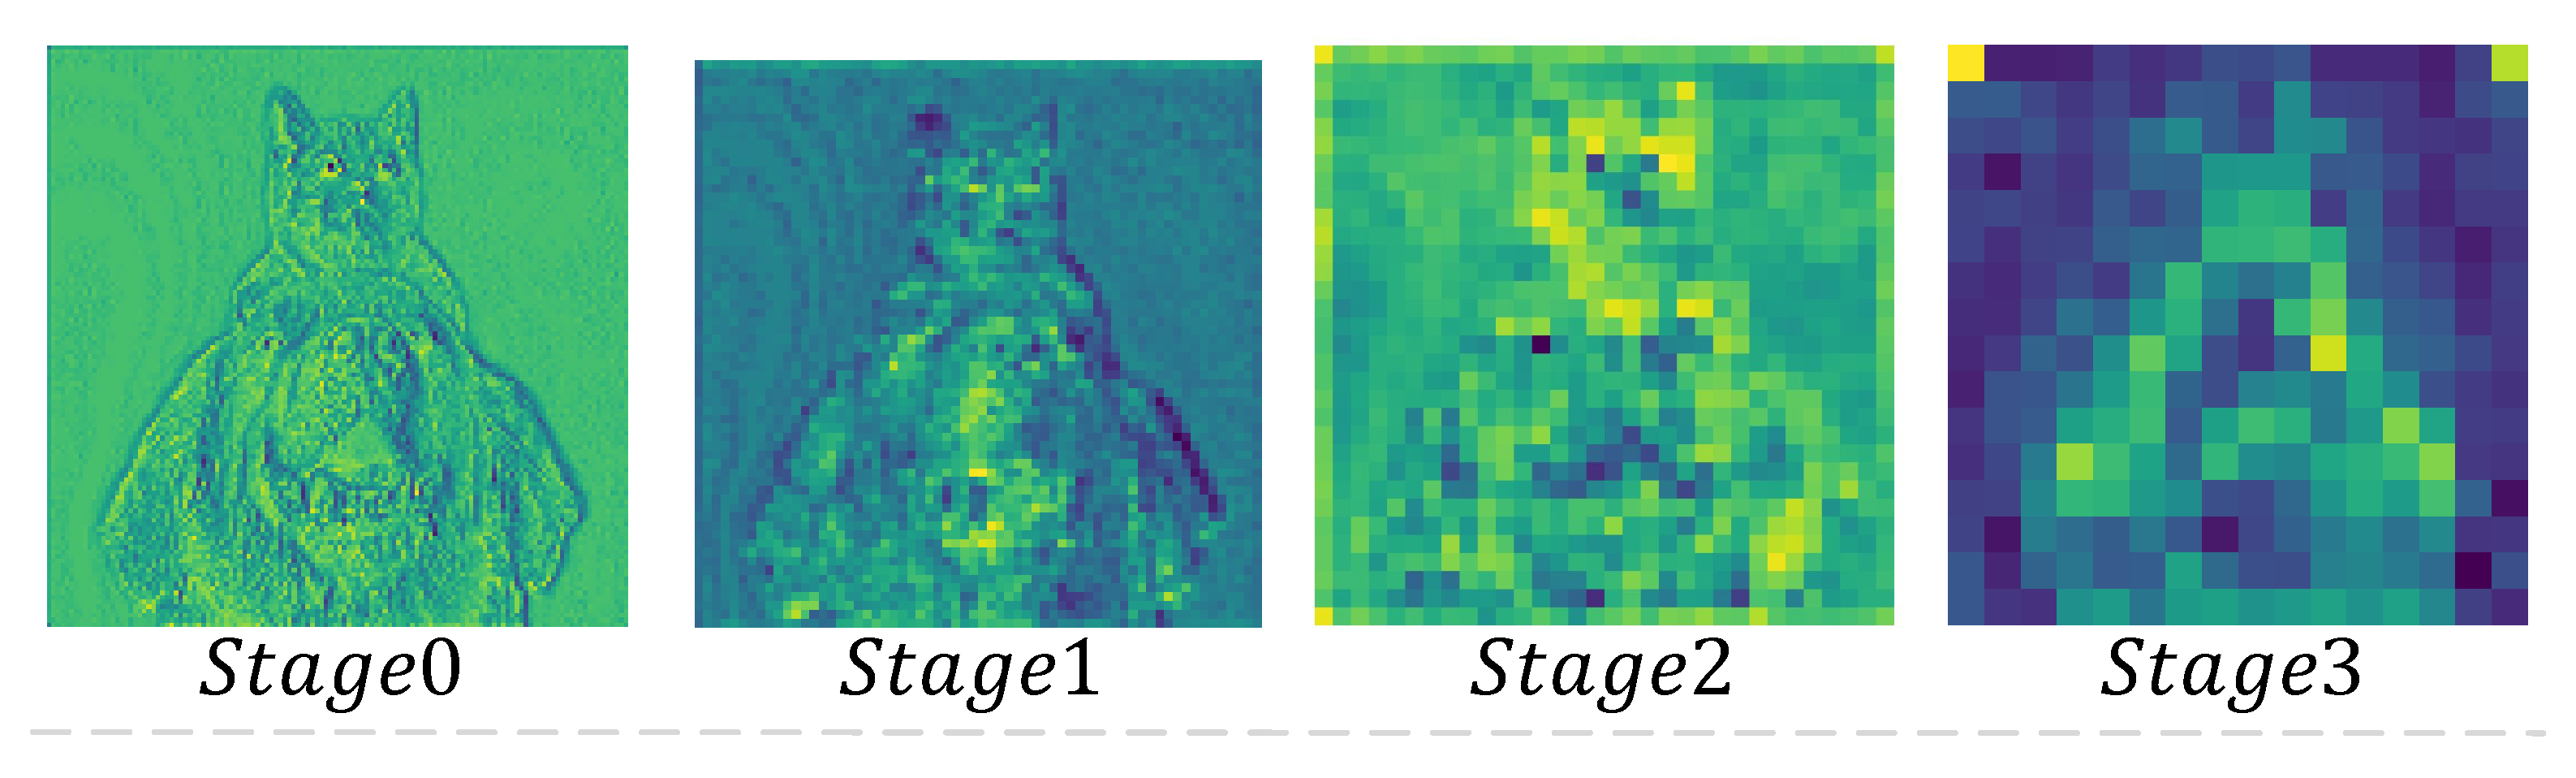
\includegraphics[width=1.\linewidth]{stages.pdf}
    \caption{Feature map evolution across network stages. Visualization of feature maps at different stages (Stage 0 to Stage 3).}
    \label{fig:stages}
\end{figure}

To achieve a more powerful spatial feature modeling capability, we propose Learnable Wavelet Spatial Attention. By using the wavelet transform~\cite{daubechies1992ten}, the feature map is converted into feature sub-bands containing different information. To enhance computational efficiency, LWSA only performs feature extraction on sub-bands that contain more information. To improve the modeling ability of key spatial features, we take advantage of the characteristic that sub-bands contain different information and construct Wavelet Spatial Attention (WSA).



% 先前的研究 \cite{finder2024wavelet,xue2023smalltrack,he2025mobilemamba} 在进行小波变换时通常依赖于预定义的固定滤波器，例如 Haar 小波 \cite{finder2022wavelet,gal2021swagan,huang2017wavelet}。经过小波变换后，输入特征图被转换为包含不同信息的四个子带。接下来，现有方法通常将这些子带沿通道维度进行拼接，然后进行特征提取 \cite{finder2024wavelet，he2025mobilemamba， ding2024wavelet}。然而，这种方法存在两个问题。首先，高层特征图包含丰富的语义信息，如图 \ref{fig：stages} 顶部所示。固定滤波器无法有效分离高层特征图的信息。其次，如图 \ref{fig：wt} 所示，小波变换后的子带包含不同方向的信息。沿通道维度简单拼接会混淆不同子带的语义。为了解决这些问题，我们创新性地提出了可学习的小波空间注意力（LWSA）。它由以下两个部分组成。
Previous studies \cite{finder2024wavelet,xue2023smalltrack,he2025mobilemamba} often relied on predefined fixed filters when conducting wavelet transforms, such as Haar Wavelet \cite{finder2022wavelet,gal2021swagan,huang2017wavelet}. After wavelet transformation, the input feature map is transformed into four sub-bands containing different information. Next, existing methods, \chadded{\color{blue}such as WTConv~\cite{finder2024wavelet}, often extract features from all sub-bands by directly applying standard convolution operations.}However, this paradigm introduces two major limitations. First, high-level feature maps contain rich semantic information, as shown in Fig.\ref{fig:stages}. Fixed filters cannot effectively separate the information of high-level feature maps. Second, existing convolution-based feature extraction methods cannot achieve a powerful spatial feature modeling capability. To solve these problems, we innovatively propose learnable wavelet spatial attention (LWSA). It consists of the following two components.

To overcome the first problem, we propose the Learnable Wavelet Basis. 
Furthermore, we construct \textbf{Learnable Wavelet Filters (LWF)} to replace the fixed filters.
This not only satisfies orthogonality but also enhances the filter's adaptability.
Given an input feature map $X \in \mathbb{R}^{C \times H \times W}$,
network generate a two-dimensional wavelet filters group $F \in \mathbb{R}^{4 \times 2 \times 2}$ for each channel slice $x \in \mathbb{R}^{1 \times H \times W}$.
Specifically, we first initialize $c$ one-dimensional learnable low-pass filters $g_{lo} \in \mathbb{R}^2 $.
The corresponding $c$ high-pass filters $g_{hi}$ are explicitly constructed according to the orthogonality condition:
\begin{equation}
\label{con:1d_filter}
\begin{aligned}
      g_{lo}^\text{init} = \frac{1}{\sqrt{2}}  \begin{bmatrix} 1 & 1 \end{bmatrix} , g_{hi} = \begin{bmatrix} g_{lo}[1] & -g_{lo}[0] \end{bmatrix}. \\
\end{aligned}
\end{equation}
Building upon this, we construct a two-dimensional analysis filter group $F$ through the matrix multiplication operation:
\begin{equation}
  \begin{split}
    F = \begin{bmatrix}F_{\text{LL}}  F_{\text{LH}} F_{\text{HL}} F_{\text{HH}} \end{bmatrix} \\
     F_{\text{LL}} = g_{\text{lo}} \otimes g_{\text{lo}}, \quad
     F_{\text{LH}} = g_{\text{lo}} \otimes g_{\text{hi}}, \\
     F_{\text{HL}} = g_{\text{hi}} \otimes g_{\text{lo}}, \quad
     F_{\text{HH}} = g_{\text{hi}} \otimes g_{\text{hi}}.
  \end{split}
% \begin{split}
%     F_{\text{LL}} = g_{\text{lo}} \otimes g_{\text{lo}}, \quad
%     F_{\text{LH}} = g_{\text{lo}} \otimes g_{\text{hi}}, \\
%     F_{\text{HL}} = g_{\text{hi}} \otimes g_{\text{lo}}, \quad
%     F_{\text{HH}} = g_{\text{hi}} \otimes g_{\text{hi}}.
% \end{split}
\end{equation}
To efficiently implement multi-channel wavelet decomposition, 
we integrate the $c$ two-dimensional filter groups into a single depthwise separable convolution kernel $W^{DW} \in \mathbb{R}^{4c \times 1 \times 2 \times 2}$.
During the backward pass, $g_{lo}$ is updated by gradient descent. Meanwhile, $g_{hi}$ and $W^{DW}$ are dynamically generated from $g_{lo}$ through orthogonality constraints and tensor operations \chadded{,  which avoids the gradient instability and divergence issues caused by non-orthogonality. } \chadded{ \color{blue}A similar hard-constraint design is also reflected in other domains to ensure optimization stability and theoretical validity~\cite{jung2025vulnerability}.}

\begin{figure} [pos=h]
    \centering
    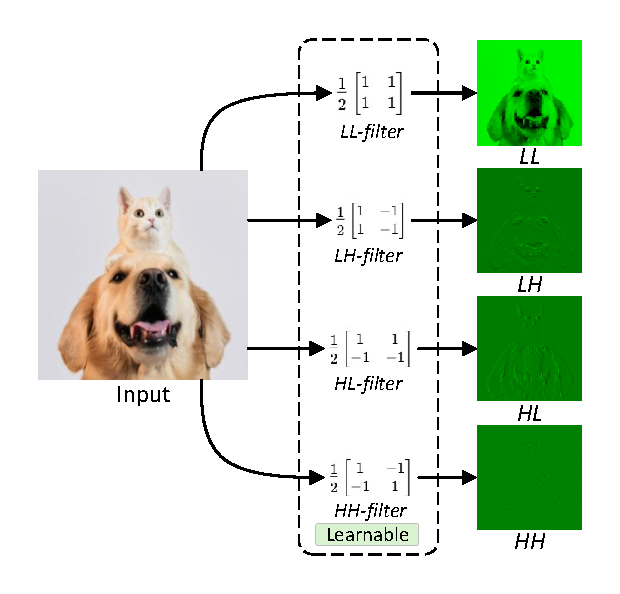
\includegraphics[width=1.\linewidth]{Wavelet_Transform.pdf}
    \caption{The process of Wavelet Transform.}
    \label{fig:wt}
\end{figure}
To fix the second problem, we propose \textbf{Wavelet Spatial Attention} to replace sample concatenation and convolutions. As shown in Fig.\ref{fig:wt}, the LL sub-band retains the most details of the input feature map. The LH sub-band and HL sub-band highlight the vertical and horizontal information, respectively. Therefore, we enhance the information of the LL sub-band by utilizing the information of the LH and HL sub-bands. Fig.\ref{fig:WCANet} (c) shows the specific operation. We first perform local convolutional feature extraction on HL and LH by leveraging DWConv, and then perform the Hadamard product \footnote{{\color{blue}Here, the symbol $\odot$ strictly denotes element-wise multiplication.}} on the two obtained feature maps. Finally, the HardSigmoid activation function is used to generate the spatial attention matrix $A$.
\begin{equation}
\begin{gathered}
    \tilde{\text{LH}} = \text{DWConv}_{3\times3}(\text{LH})\\
    \quad \tilde{\text{HL}} = \text{DWConv}_{3\times3}(\text{HL}) \\
    A = \text{Hardsigmoid}\left( \tilde{\text{LH}} \odot \tilde{\text{HL}} \right)
\end{gathered}
\end{equation}
where the shape of $A \in \mathbb{R}^{B \times C \times H/2 \times W/2} $ is the same as that of the LL sub-band. Thus, spatial attention is achieved through the operation as shown in the formula X:
\begin{equation}
\tilde{\text{LL}}_{\text{attn}} = A \odot \text{DWConv}_{k\times k}(\text{LL}) + \text{LL},
\end{equation}
where k represents the size of the convolution kernel. Its value can be dynamically set according to the stage of the network $\big(Stage 0:(k=7), Stage 1:(k=5), Stage \geq2:(k=3)\big)$.
\begin{equation}
IWT(\tilde{\text{LL}}_{\text{attn}},\tilde{\text{LH}},\tilde{\text{HL}},HH)=X^\text{out}
\end{equation}
We concatenate $\tilde{\text{LL}}_{\text{attn}}$,$\tilde{\text{LH}}$,$\tilde{\text{HL}}$ with the original $\text{HH}$ along the channel-wise, and then perform an inverse wavelet transform to restore the feature map to its original size. 







\subsection{The design of WCANet}





 We present the lightweight model design, i.e., WCANet, as shown in Fig.\ref{fig:WCANet}. It uses a sequence attention as the primary operation. We present
the basic block, i.e., CCSA block in Fig.\ref{fig:WCANet} (b).



\begin{figure*} [pos=t]
    \centering
    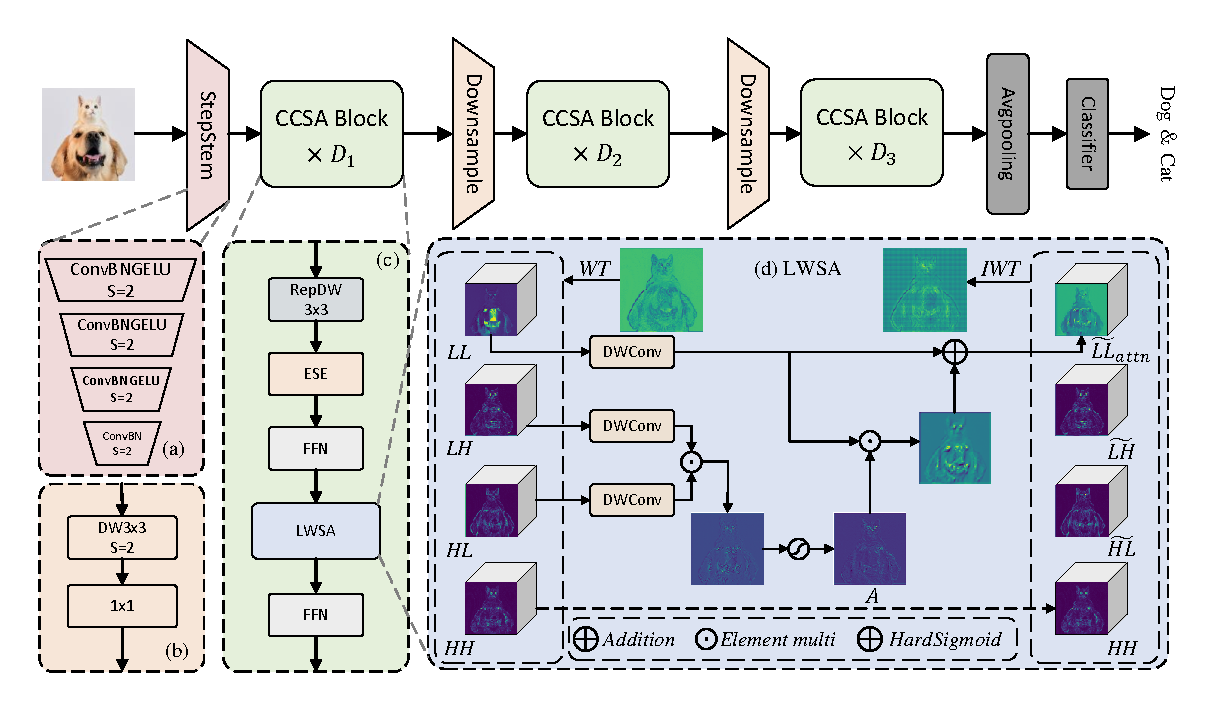
\includegraphics[width=0.9\linewidth]{WCANet.pdf}
    \caption{The structure of WCANet. (a) is the StepStem. (b) is the CCSA Block. (c) is the LWSA.}
    \label{fig:WCANet}
\end{figure*}


CCSA block applies attention operations separately along the channel and spatial dimensions, which achieves a powerful feature extraction capability. In the channel dimension, the ESE module is employed to suppress redundant channels and enhance effective channels. In the spatial dimension, we employ LWSA to achieve effective spatial feature extraction. Besides, we utilize the extra depthwise convolution and FFN to enhance the model's capability.



\begin{table} [pos=h]
  \caption{Comparison of WCANet architectures with different total downsampling ratios: WCANet-T4×32 and WCANet-T5x32 denote 4-stage networks with a total downsampling factor of 32, while WCANet-T4×64 and WCANet-T5×64 denote 3-stage networks with a total downsampling factor of 64.}
  \label{tab:compare_64_32}
  \centering
  \begin{tabular}{lccc}
    \toprule
    \makecell{model} & \makecell{network \\ structure} & \makecell{Throughput \\ (images/s)} &  \makecell{FLOPs \\ (M)}  \\
    \midrule
    \makecell{ WCANet-T4 \\ $\times32$} & \makecell{$\{32,64,128,256\}$ \\ $\{1,2,4,5\}$}  & 5334 & 275  \\
    \makecell{ WCANet-T4 \\ $\times64$} & \makecell{$\{128,256,512\}$ \\ $\{2,3,2\}$}  & 9921 & 313  \\ 
    \midrule
    \makecell{ WCANet-T5 \\ $\times32$} & \makecell{$\{40,80,160,320\}$ \\ $\{1,2,4,5\}$}  & 4112 & 442  \\
    \makecell{ WCANet-T5 \\ $\times64$} & \makecell{$\{128,256,512\}$ \\ $\{3,4,3\}$}  & 7472 & 410  \\ 
    \bottomrule
  \end{tabular}
\end{table}

We compare the $\times32$ and $\times64$ downsampling multi-stage architectures. 
As shown in Tab \ref{tab:compare_64_32}, under different network architectures, $\times64$ downsampling is more efficient than $\times32$ downsampling. Furthermore, the experimental results show that WCANet-T4×64 achieves a Top-1 accuracy $0.8\uparrow$ than its $\times32$ counterpart, and WCANet-T5×64 matches the Top-1 accuracy of the $\times32$ version. Therefore, we utilize the 64× downsampling in WCANet. 

Overall, WCANet employs a StepStem \cite{xiao2021early} to project the input image into the visual feature map. For
downsampling, we leverage the depth-wise and point-wise
convolution to reduce the spatial resolution and modulate
the channel dimension, respectively. Besides, we stack CCSA blocks in all stages. Finally, the feature map is processed by global average pooling and a classifier to produce the final class prediction.

We build multiple WCANet variants to accommodate different computational budgets. Under an input resolution of 256×256, their FLOPs range from 80M to 650M, namely WCANet-T0, WCANet-T1, WCANet-T2, WCANet-T2P5, WCANet-T3, WCANet-T4, WCANet-T5, and WCANet-T6. Additionally, to better suit downstream dense prediction tasks, we also design a four-stage WCANet variant with 64× downsampling: WCANet-T8.


































\begin{table} [pos=t]
  \caption{Classification results of different models on ImageNet-1K. } 
  \label{tab:imagenet}
  \setlength{\tabcolsep}{2pt}
  \small
  \centering
  \begin{tabular}{lcccccc}
  \toprule
  Model & \makecell{Params\\(M)} & \makecell{FLOPs\\(M)} & \makecell{Reso.} & \makecell{Top-1\\(\%)} & {\#Pub} \\
  \toprule
{EfficientViT-M0~\cite{liu2023efficientvit}} & 2.3 & 79 & 224 & 63.2 & CVPR'23\\
{MobileNetv3-Lx035~\cite{howard2019searching}} & 2.1 & 77 & 224 & 64.2 & ICCV'19 \\

\rowcolor[gray]{0.92}
\textbf{WCANet-T1} & 2.0 & 78 & 256 & 64.5 & - \\
\rowcolor[gray]{0.92}
\textbf{WCANet-T2} & 2.5 & 102 & 256 & \textbf{66.7} & - \\

\midrule

{EfficientViT-M1~\cite{liu2023efficientvit}} & 3.0 & 167 & 224 & 68.4 & CVPR'23\\
{MobileNetv3Lx05~\cite{howard2019searching}} & 2.6 & 138 & 224 & 68.8 & ICCV'19 \\
{ShufflenetV2-1.0x~\cite{ma2018shufflenet}} & 2.3 & 146 & 224 & 69.4 & ECCV'18 \\
{EfficientViT-M2~\cite{liu2023efficientvit}} & 4.2 & 201 & 224 & 70.8 & CVPR'23\\
\rowcolor[gray]{0.92}
\textbf{WCANet-T2d5} & 3.7 & 151 & 256 & 70.3 & - \\
\rowcolor[gray]{0.92}
\textbf{WCANet-T3} & 5.1 & 208 & 256 & \textbf{72.3} & - \\

\midrule
  EdgeNeXt-XXS~\cite{maaz2022edgenext} & 1.3 & 260 &224 &71.2 & ECCV'22 \\
  FasterNet-T0~\cite{chen2023run} & 3.9 & 340 & 224 & 71.9  & CVPR'23 \\
  ShuffleNetV2-1.5x~\cite{ma2018shufflenet} & 3.5 & 300 & 224 & 72.6 & ECCV'18 \\
  EMO-1M~\cite{zhang2023rethinking} & 1.3 & 261 & 224 & 71.5 & ICCV'23 \\
  SHViT-S1~\cite{yun2024shvit} & 6.3 & 241 & 224 & 72.8 & CVPR'24 \\
{EfficientViT-M3~\cite{liu2023efficientvit}} & 6.9 & 263 & 224 & 73.4 & CVPR'23\\
  StarNet-S1~\cite{ma2024rewrite} & 2.9 & 425 & 224 & 73.5 & CVPR'24 \\
  MobileMamba-T2~\cite{he2025mobilemamba} & 8.8 & 255 & 192 & 73.6 & CVPR'25 \\
  {EfficientViT-M4~\cite{liu2023efficientvit}} & 8.8 & 299 & 224 & 74.3 & CVPR'23\\
  LSNet-T~\cite{wang2025lsnet} & 11.4 & 320 & 224 & 74.9 & CVPR'25  \\
  EMO-2M~\cite{zhang2023rethinking} & 2.3 & 439 & 224 & 75.1 & ICCV'23 \\
  SHViT-S2~\cite{yun2024shvit} & 11.4 & 366 & 224 & 75.2 & CVPR'24 \\
  MobileMamba-T4~\cite{he2025mobilemamba} & 14.2 & 413 & 192 & 76.1 & CVPR'25 \\
  \rowcolor[gray]{0.92}
\textbf{WCANet-T4} & 7.6 & 313 & 256 & 74.9 & - \\
  \rowcolor[gray]{0.92}
\textbf{WCANet-T5} & 10.8 & 410 & 256 & \textbf{76.8} & - \\
  \midrule
  StarNet-S2~\cite{ma2024rewrite} & 3.7 & 547 & 224 & 74.7 & CVPR'24 \\
EdgeNeXt-XS~\cite{maaz2022edgenext} & 2.3 & 540 & 224 & 75.0 & ECCV'22\\
FasterNet-T1~\cite{chen2023run} & 7.6 & 850 & 224 & 76.2  & CVPR'23 \\
{EfficientViT-M5~\cite{liu2023efficientvit}} & 12.4 & 522 & 224 & 77.1 & CVPR'23\\
SHViT-S3~\cite{yun2024shvit} & 14.2 & 601 & 224 & 77.4 & CVPR'24 \\
MobileMamba-S6~\cite{he2025mobilemamba} & 15.0 & 652 & 224 & 78.0 & CVPR'25 \\
\rowcolor[gray]{0.92}
\textbf{WCANet-T6} & 16.5 & 644 & 256 & \textbf{78.2} & - \\
  \midrule
StarNet-S3~\cite{ma2024rewrite} & 5.8 & 757 & 224 & 77.4 & CVPR'24 \\
RepViT-M0.9~\cite{wang2024repvit} & 5.1 & 846 & 224 & 77.4 & CVPR'24 \\
EdgeViT-XS~\cite{pan2022edgevits} & 6.7 & 1100 & 224 & 77.5 & ICCV'22 \\
StarNet-S4~\cite{ma2024rewrite} & 7.5 & 1075 & 224 & 78.8 & CVPR'24 \\
FasterNet-T2~\cite{chen2023run} & 15.0 & 1917 & 224 & 78.9  & CVPR'23 \\
EMO-6M~\cite{zhang2023rethinking} & 6.1 & 961 & 224 & 79.0 & ICCV'23 \\
SHViT-S4~\cite{yun2024shvit} & 16.5 & 986 & 256 & 79.4 & CVPR'24 \\
{EfficientViT-M4~\cite{liu2023efficientvit}} & 12.4 & 1486 & 384 & 79.8 & CVPR'23\\
MobileMamba-B1~\cite{he2025mobilemamba} & 17.1 & 1080 & 256 & 79.9 & CVPR'25 \\
\rowcolor[gray]{0.92}
\textbf{WCANet-T8} & 26.0 & 1078 & 256 & \textbf{80.0} & - \\
  \bottomrule
  \end{tabular}
  \vspace{-10pt}
\end{table}



\section{Experiments}


\subsection{Image Classification}

% We conduct experiments on the ImageNet-1K~\cite{deng2009imagenet} dataset to evaluate the performance of WCANet on the image classification task. 
% \chadded{To ensure a fair and rigorous comparison against baselines spanning different publication years, we explicitly document our training protocol. Specifically, WCANet is trained entirely from scratch without relying on Knowledge Distillation (KD), additional pre-training datasets, or multi-scale training procedures. The detailed hyperparameters and data augmentation strategies are fully documented in Table~\ref{tab:train_detail}.} 
% The overall training protocol is similar to that of~\cite{liu2023efficientvit,wang2025lsnet,he2025mobilemamba}, {.............}except that WCANet uses an input image resolution of $256 \times 256$ and a learning rate that is cosine-annealed from 3e-3 to 1e-5.

We conduct experiments on the ImageNet-1K~\cite{deng2009imagenet} dataset to evaluate the performance of WCANet on the image classification task. \chadded{To ensure a fair and rigorous comparison against baselines spanning different publication years, we explicitly document our training protocol. Specifically, WCANet is trained entirely from scratch without relying on Knowledge Distillation (KD), additional pre-training datasets, or multi-scale training procedures. The detailed hyperparameters and data augmentation strategies are fully documented in Table~\ref{tab:train_detail}.} The overall training protocol is similar to that of~\cite{liu2023efficientvit,wang2025lsnet,he2025mobilemamba}, except that WCANet uses an input image resolution of $256 \times 256$ and a learning rate that is cosine-annealed from 3e-3 to 1e-5. \chadded{As WCANet incorporates wavelet transform mechanisms across multiple stages, the maximum downsampling factor of the network reaches 128. To ensure the complete alignment of feature dimensions, the input resolution must be perfectly divisible by this factor. Therefore, WCANet uses an input image resolution of $256 \times 256$.}


Table~\ref{tab:imagenet} shows the performance of WCANet, compared with other state-of-the-art (SoTA) methods under similar model scales. The different model scales are categorized by FLOPs. Compared with CNNs, WCANet demonstrates consistently superior performance at the same computational cost. Specifically, WCANet-T4 outperforms FasterNet-T0~\cite{chen2023run} by $+3\uparrow$. WCANet-T8 surpasses FasterNet-T2~\cite{chen2023run} by $1.1\uparrow$ in Top-1 while having only 56\% of its FLOPs. Furthermore, WCANet variants consistently surpass StarNet~\cite{ma2024rewrite} counterparts by $1.2\uparrow$ to $3.3\uparrow$ in Top-1. Compared with ViTs, ViMs, and hybrid architectures, WCANet also demonstrates strong competitiveness. Under comparable FLOPs, 

WCANet variants consistently outperform the Transformer-based EfficientViT~\cite{liu2023efficientvit} series in Top-1 accuracy. WCANet-T4 achieves 74.9\% Top-1 accuracy, surpassing the Mamba-based MobileMamba-T2~\cite{he2025mobilemamba} by $+1.3\uparrow$. At approximately 1 GFLOPs, WCANet-T8 achieves 80.0\% Top-1 accuracy, outperforming contemporary architectures at similar computational costs, including MobileMamba-B1~\cite{he2025mobilemamba}, EMO-6M~\cite{zhang2023rethinking}, and ShViT-S4~\cite{yun2024shvit}. These experimental results strongly indicate that by employing LWSA for spatial feature extraction and the ESE module for inter-channel information fusion, the proposed model performs very well in terms of classification accuracy.











\begin{table}[pos=t]
\caption{{\color{blue}
\textbf{Comparison with SoTAs in inference efficiency.}
GPU throughput is measured on an NVIDIA GeForce RTX 4090 with a batch size of 2048;
CPU throughput is evaluated on an Intel(R) Xeon(R) Platinum 8352V with a batch size of 16;
and ARM throughput is evaluated on an Apple M1 chip with a batch size of 8.
Each model is evaluated at the input resolution listed in the ``Reso.'' column.
Throughput is reported as mean $\pm$ standard deviation over five repeated runs.
}}
  \vspace{-0.2cm}
  \centering
  \renewcommand{\arraystretch}{1.0}
  \setlength\tabcolsep{3.5pt} % 稍微收缩间距以适应单栏
  \resizebox{1\linewidth}{!}{
  \begin{tabular}{lccccccc}
    \toprule
    \multirow{2}[4]{*}{Model} & \multicolumn{1}{c}{FLOPs} & \multicolumn{1}{c}{\#Params} & \multirow{2}[4]{*}{Reso.} & \multicolumn{3}{c}{Throughput (img/s)} & \multirow{2}[4]{*}{Top-1 \%} \\
    \cmidrule{5-7}          &   (M)    &   (M)    &       & GPU   & CPU   & ARM & \\
    \midrule
    StarNet-S1 & 425 & 2.9 & 224 & 6898$\pm$55 & 42.7$\pm$0.8 & 25.8$\pm$0.5 & 73.5\\
    FasterNet-T0 & 340 & 3.9 & 224 & 15682$\pm$141 & 77.4$\pm$1.2 & 62.6$\pm$1.0 & 71.9\\
    MobileMamba-T2 & 255 & 8.8 & 192 & 19541$\pm$127 & 54.6$\pm$1.0 & 51.7$\pm$0.9 & 73.6\\
    LSNet-T & 320 & 11.4 & 224 & 16106$\pm$134 & - & - & 74.9 \\
      \rowcolor[gray]{0.92}
    \textbf{WCANet-T4} & 313 & 7.6 & 256 & 20274$\pm$146 & 60.6$\pm$1.1 & 48.7$\pm$0.8 & 74.9 \\
    \midrule
    FasterNet-T1 & 850 & 7.6 & 224 & 10731$\pm$163 & 38.7$\pm$0.7 & 42.6$\pm$0.8 & 76.2\\
    MobileMamba-T4 & 413 & 14.2 & 192 & 15418$\pm$128 & 40.7$\pm$0.8 & 38.8$\pm$0.7 & 76.1\\
      \rowcolor[gray]{0.92}
    \textbf{WCANet-T5} & 410 & 10.8 & 256 & 15241$\pm$143 & 41.7$\pm$1.4 & 34.8$\pm$0.6 & 76.8 \\
    \midrule
    FasterNet-T2 & 1917 & 15.0 & 224 & 4946$\pm$95 & 18.8$\pm$0.8 & 27.7$\pm$0.6 & 78.9\\
    StarNet-S4 & 1075 & 7.5 & 224 & 3492$\pm$43 & 23.8$\pm$0.5 & 11.9$\pm$0.4 & 78.8\\
    MobileMamba-B1 & 1080 & 17.1 & 256 & 6152$\pm$52 & 12.8$\pm$0.4 & 15.8$\pm$0.7 & 79.9\\
      \rowcolor[gray]{0.92}
    \textbf{WCANet-T8} & 1078 & 26.0 & 256 & 6236$\pm$57 & 17.8$\pm$0.4 & 16.8$\pm$0.3 & 80.0 \\
    \bottomrule
  \end{tabular}%
  }
  \label{tab:efficiency}%
\end{table}



% \subsection{Efficiency Comparison}




\begin{table*}[pos=t]
\caption{\textbf{Object detection and instance segmentation results on COCO.} AP$^{\rm b}$ and AP$^{\rm m}$ indicate bounding box AP and mask AP, respectively. 
\chadded{\color{blue}For a fair comparison, all baselines are evaluated according to the training protocols reported in their original publications.}
}
\label{tab:coco} 
\centering
\small
\resizebox{\textwidth}{!}{
\begin{tabular}{l|ccc|ccc|ccc|ccc}
  \toprule
  \multirow{2}{*}{Backbone} & \multicolumn{6}{c|}{RetinaNet} & \multicolumn{6}{c}{Mask R-CNN} \\ 
  \cmidrule{2-13}
  & AP & AP$_{50}$ & AP$_{75}$ & AP$_S$ & AP$_M$ & AP$_L$ & AP$^{\rm b}$ & AP$_{50}^{\rm b}$ & AP$_{75}^{\rm b}$ & AP$^{\rm m}$ & AP$_{50}^{\rm m}$ & AP$_{75}^{\rm m}$ \\
  \toprule 
  EfficientViT-M5~\cite{liu2023efficientvit} & 34.3 & 54.2 & 36.1 & 18.0 & 36.9 & 48.2 & 34.9 & 57.0 & 37.0 & 32.8 & 53.7 & 34.6 \\
  SHViT-S3~\cite{yun2024shvit} & 36.1 & 56.6 & 38.0 & 19.9 & 39.1 & 50.8 & 36.9 & 59.4 & 39.6 & 34.4 & 56.3 & 36.1 \\
  ResNet50~\cite{he2016deep} & 36.3 & 55.3 & 38.6 & 19.3 & 40.0 & 48.8 & 38.0 & 58.6 & 41.4 & 34.4 & 55.1 & 36.7\\
  PVT-Tiny~\cite{wang2021pyramid} & 36.7 & 56.9 & 38.9 & \textbf{22.6} & 38.8 & 50.0  & 36.7 & 59.2 & 39.3 & 35.1 & 56.7 & 37.3 \\
  PoolFormer-S12~\cite{yu2022metaformer} & 36.2 & 56.2 & 38.2 & 20.8 & 39.1 & 48.0 & 37.3 & 59.0 & 40.1 & 34.6 & 55.8 & 36.9\\
    LSNet-S~\cite{wang2025lsnet} & 36.7 & 67.2 & 38.6 & 20.0 & 39.7 & 51.8 & 37.4 & 59.9 &39.8 & 34.8 & 56.8 & 36.6 \\
  FasterNet-S~\cite{chen2023run} & - & - & - & - & - & - & 39.9 & 61.2 & \textbf{43.6} & \textbf{36.9} & 58.1 & \textbf{39.7}  \\
  \rowcolor[gray]{0.92}
   \textbf{WCANet-T8} & \textbf{38.6} & \textbf{59.0} & \textbf{41.1} & 22.5 & \textbf{41.5} & \textbf{51.7} & \textbf{40.0} & \textbf{61.3} & 43.4 & 36.7 & \textbf{58.6} & 39.1 \\
  \bottomrule
\end{tabular}
}
\vspace{-10pt}
\end{table*}
\begin{figure*}[pos=t] 
    \centering
    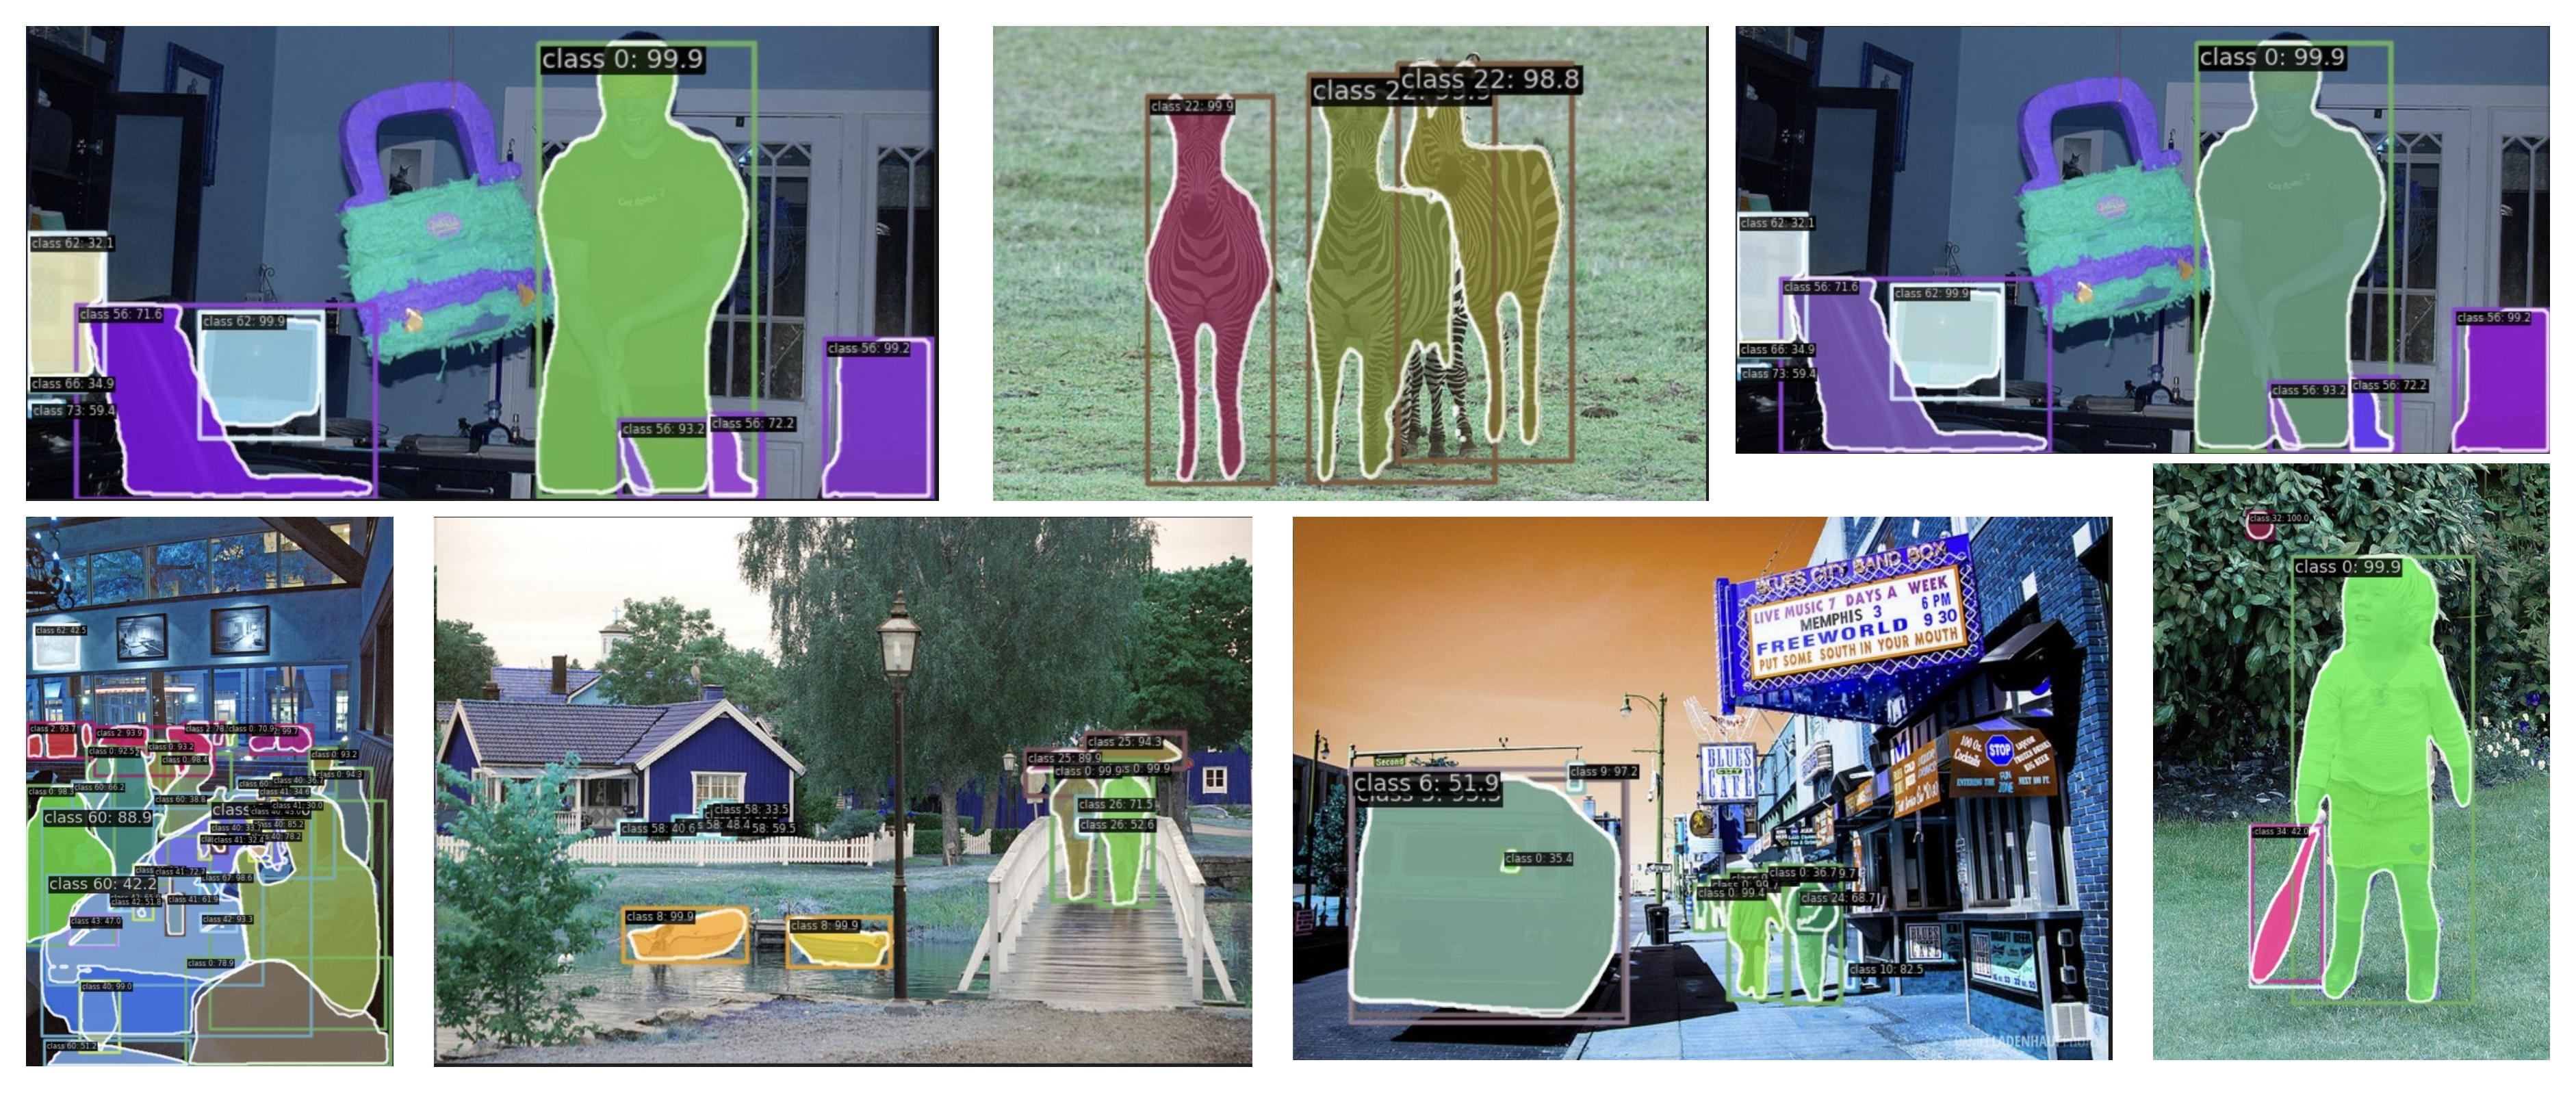
\includegraphics[width=0.95\linewidth]{visualization.pdf}
    \caption{\chadded{\color{blue}Qualitative results for object detection and instance segmentation on COCO-2017 using WCANet as the backbone framework.}}
    \label{fig:COCO_vis}
\end{figure*}



\subsection{Inference Efficiency Analysis}
\label{sec:efficiency}

{ \color{blue}
To demonstrate the hardware-aware efficiency of WCANet, we conduct comprehensive throughput evaluations across three diverse hardware platforms: NVIDIA GeForce RTX 4090 (GPU), Intel Xeon Platinum 8352V (CPU), and Apple M1 (ARM-based chip). All throughput metrics are reported in images per second (img/s) with a batch size of 8 to ensure consistency.

As summarized in Table \ref{tab:efficiency}, WCANet consistently outperforms existing state-of-the-art models across all tested platforms. Specifically, on the GPU platform, WCANet-T4 achieves a throughput of 20,388 img/s, significantly surpassing MobileMamba-T2 while maintaining competitive Top-1 accuracy. More importantly, our model demonstrates robust scalability on constrained devices. On the Apple M1 chip, WCANet-T8 maintains an efficient throughput of 17 img/s while achieving a top-1 accuracy of 80.0\%, showcasing its architectural superiority for mobile and edge deployment.

The performance trade-offs are further visualized in Figure \ref{fig:GPU_throught}, which plots the relationship between inference latency/throughput and Top-1 accuracy. As illustrated, WCANet consistently resides on the upper-left or lower-right frontier of the Pareto curves compared to FasterNet, StarNet, and MobileMamba. This indicates that WCANet effectively balances the feature extraction capability of learnable wavelet filters with the computational overhead, providing a distinct advantage for real-time applications where both accuracy and hardware-specific latency are critical constraints.
}

% \subsection{WCANet on Downstream Tasks}







\subsection{Object Detection and Segmentation on COCO}

To further evaluate the generalization ability of WCANet, we conduct object detection and instance segmentation experiments on the COCO dataset~\cite{lin2014microsoft}.
We first pre-train the WCANet in ImageNet-1k, and then use it as the backbone integrated with both RetinaNet~\cite{lin2017focal} and Mask R-CNN~\cite{he2017mask} frameworks.
The models are trained for 12 epochs (1× schedule) with a total batch size of 16, using an AdamW optimizer~\cite{loshchilov2017decoupled} (learning rate $1\times 10^{-4}$, weight decay 0.05).
The learning rate is linearly warmed up over the first 500 iterations and then decayed via cosine annealing, with gradient clipping (max norm 0.1).
No additional hyper-parameter tuning is performed.

Table \ref{tab:coco} shows the comparison between WCANet and representative models.
WCANet consistently achieves higher average precision (AP) than conventional CNN baselines under comparable model complexity.
Specifically, WCANet-T8 outperforms the standard ResNet50~\cite{he2016deep} by +2.3 $AP^b$ with RetinaNet, and by +2.0 $AP^b$ and +2.3 $AP^m$ with Mask R-CNN.
Moreover, WCANet-T8 shows competitive performance against the efficient CNN architecture FasterNet-S~\cite{chen2023run}, achieving +0.1 higher $AP^b$ (40.0 vs.39.9) but slightly lower $AP^m$ (36.7 vs.36.9) under Mask R-CNN.


\chadded{\color{blue}To provide a qualitative evaluation of the proposed network, we visualize the object detection and instance segmentation results in Fig.~\ref{fig:COCO_vis}. Notably, WCANet exhibits robust detection and precise segmentation even for small and texture-rich objects. While the LWSA module discards the HH sub-band to optimize computational efficiency, the visualization and our quantitative results (e.g., 22.5\% $AP_S$ in RetinaNet) demonstrate that the remaining LH and HL sub-bands sufficiently capture the critical high-frequency spatial details, such as edges and boundaries, required for dense prediction tasks. Therefore, WCANet successfully maintains high sensitivity to small objects while strictly bounding the computational overhead.}







% To further evaluate the generalization ability of WCANet, we conduct object detection and instance segmentation experiments on the COCO dataset~\cite{lin2014microsoft}. We first pre-train the WCANet in ImageNet-1k, and then use it as the backbone integrated with both RetinaNet~\cite{lin2017focal} and Mask R-CNN~\cite{he2017mask} frameworks. The models are trained for 12 epochs (1× schedule) with a total batch size of 16, using an AdamW optimizer~\cite{loshchilov2017decoupled} (learning rate $1\times 10^{-4}$, weight decay 0.05). The learning rate is linearly warmed up over the first 500 iterations and then decayed via cosine annealing, with gradient clipping (max norm 0.1). No additional hyper-parameter tuning is performed.


% Table \ref{tab:coco} shows the comparison between WCANet and representative models. WCANet consistently achieves higher average precision (AP) than conventional CNN baselines under comparable model complexity. Specifically, WCANet-T8 outperforms the standard ResNet50~\cite{he2016deep} by +2.3 $AP^b$ with RetinaNet, and by +2.0 $AP^b$ and +2.3 $AP^m$ with Mask R-CNN. Moreover, WCANet-T8 shows competitive performance against the efficient CNN architecture FasterNet-S~\cite{chen2023run}, achieving +0.1 higher $AP^b$ (40.0 vs.39.9) but slightly lower $AP^m$ (36.7 vs.36.9) under Mask R-CNN. 



% \begin{table*}[t]
% \centering
% \caption{Performance comparison on the ClinicDB medical imaging dataset evaluating the adaptability of learnable filters to different frequency distributions.}
% \label{tab:clinicdb_domain_adaptation}
% \begin{tabular}{lcccc}
% \toprule
% \textbf{Method} & \textbf{Val Dice (\%)} & \textbf{Val IoU (\%)} & \textbf{Test Dice (\%)} & \textbf{Test IoU (\%)} \\
% \midrule
% Baseline UNet (MK\_UNet)          & 91.13 & 85.21 & 93.38 & 88.38 \\
% WCANet (Fixed Haar Filters)       & 91.60 & 86.14 & 93.89 & 89.07 \\
% \rowcolor[gray]{0.92}
% WCANet (Learnable Filters, Ours)& \textbf{92.68} & \textbf{87.20} & \textbf{94.41} & \textbf{89.69} \\
% \bottomrule
% \end{tabular}
% \end{table*}

% \textbf{Adaptability to Other Visual Domains.} 
% To evaluate how WCANet behaves across domains where the frequency characteristics of meaningful features differ substantially from natural ImageNet statistics, we conduct further experiments on medical image segmentation using the ClinicDB dataset. Medical images often exhibit unique texture and edge distributions. As shown in Table~\ref{tab:clinicdb_domain_adaptation}, directly applying fixed Haar filters provides a marginal improvement over the baseline UNet. However, WCANet equipped with our proposed learnable wavelet filters achieves significant performance gains, reaching 94.41\% Test Dice and 89.69\% Test IoU. This demonstrates that our learnable filters, strictly guided by the orthogonality constraint, can stably and effectively adapt to severe distribution shifts without collapsing. The orthogonality constraint ensures that the dynamic decomposition remains mathematically sound even when optimizing for highly specific, non-natural frequency distributions.




\begin{table*}[pos=t]
\centering
\caption{\chadded{Performance comparison on the ClinicDB medical imaging dataset evaluating the adaptability of learnable filters to different frequency distributions.}}
\label{tab:clinicdb_domain_adaptation}
\begin{tabular}{lcccc}
\toprule
\textbf{Method} & \textbf{Val Dice (\%)} & \textbf{Val IoU (\%)} & \textbf{Test Dice (\%)} & \textbf{Test IoU (\%)} \\
\midrule
Baseline UNet (MK\_UNet)          & 91.13 & 85.21 & 93.38 & 88.38 \\
WCANet (Fixed Haar Filters)       & 91.60 & 86.14 & 93.89 & 89.07 \\
\rowcolor[gray]{0.92}
WCANet (Learnable Filters, Ours)  & \textbf{92.68} & \textbf{87.20} & \textbf{94.41} & \textbf{89.69} \\
\bottomrule
\end{tabular}
\end{table*}

\begin{figure*} [pos=h]
    \centering
    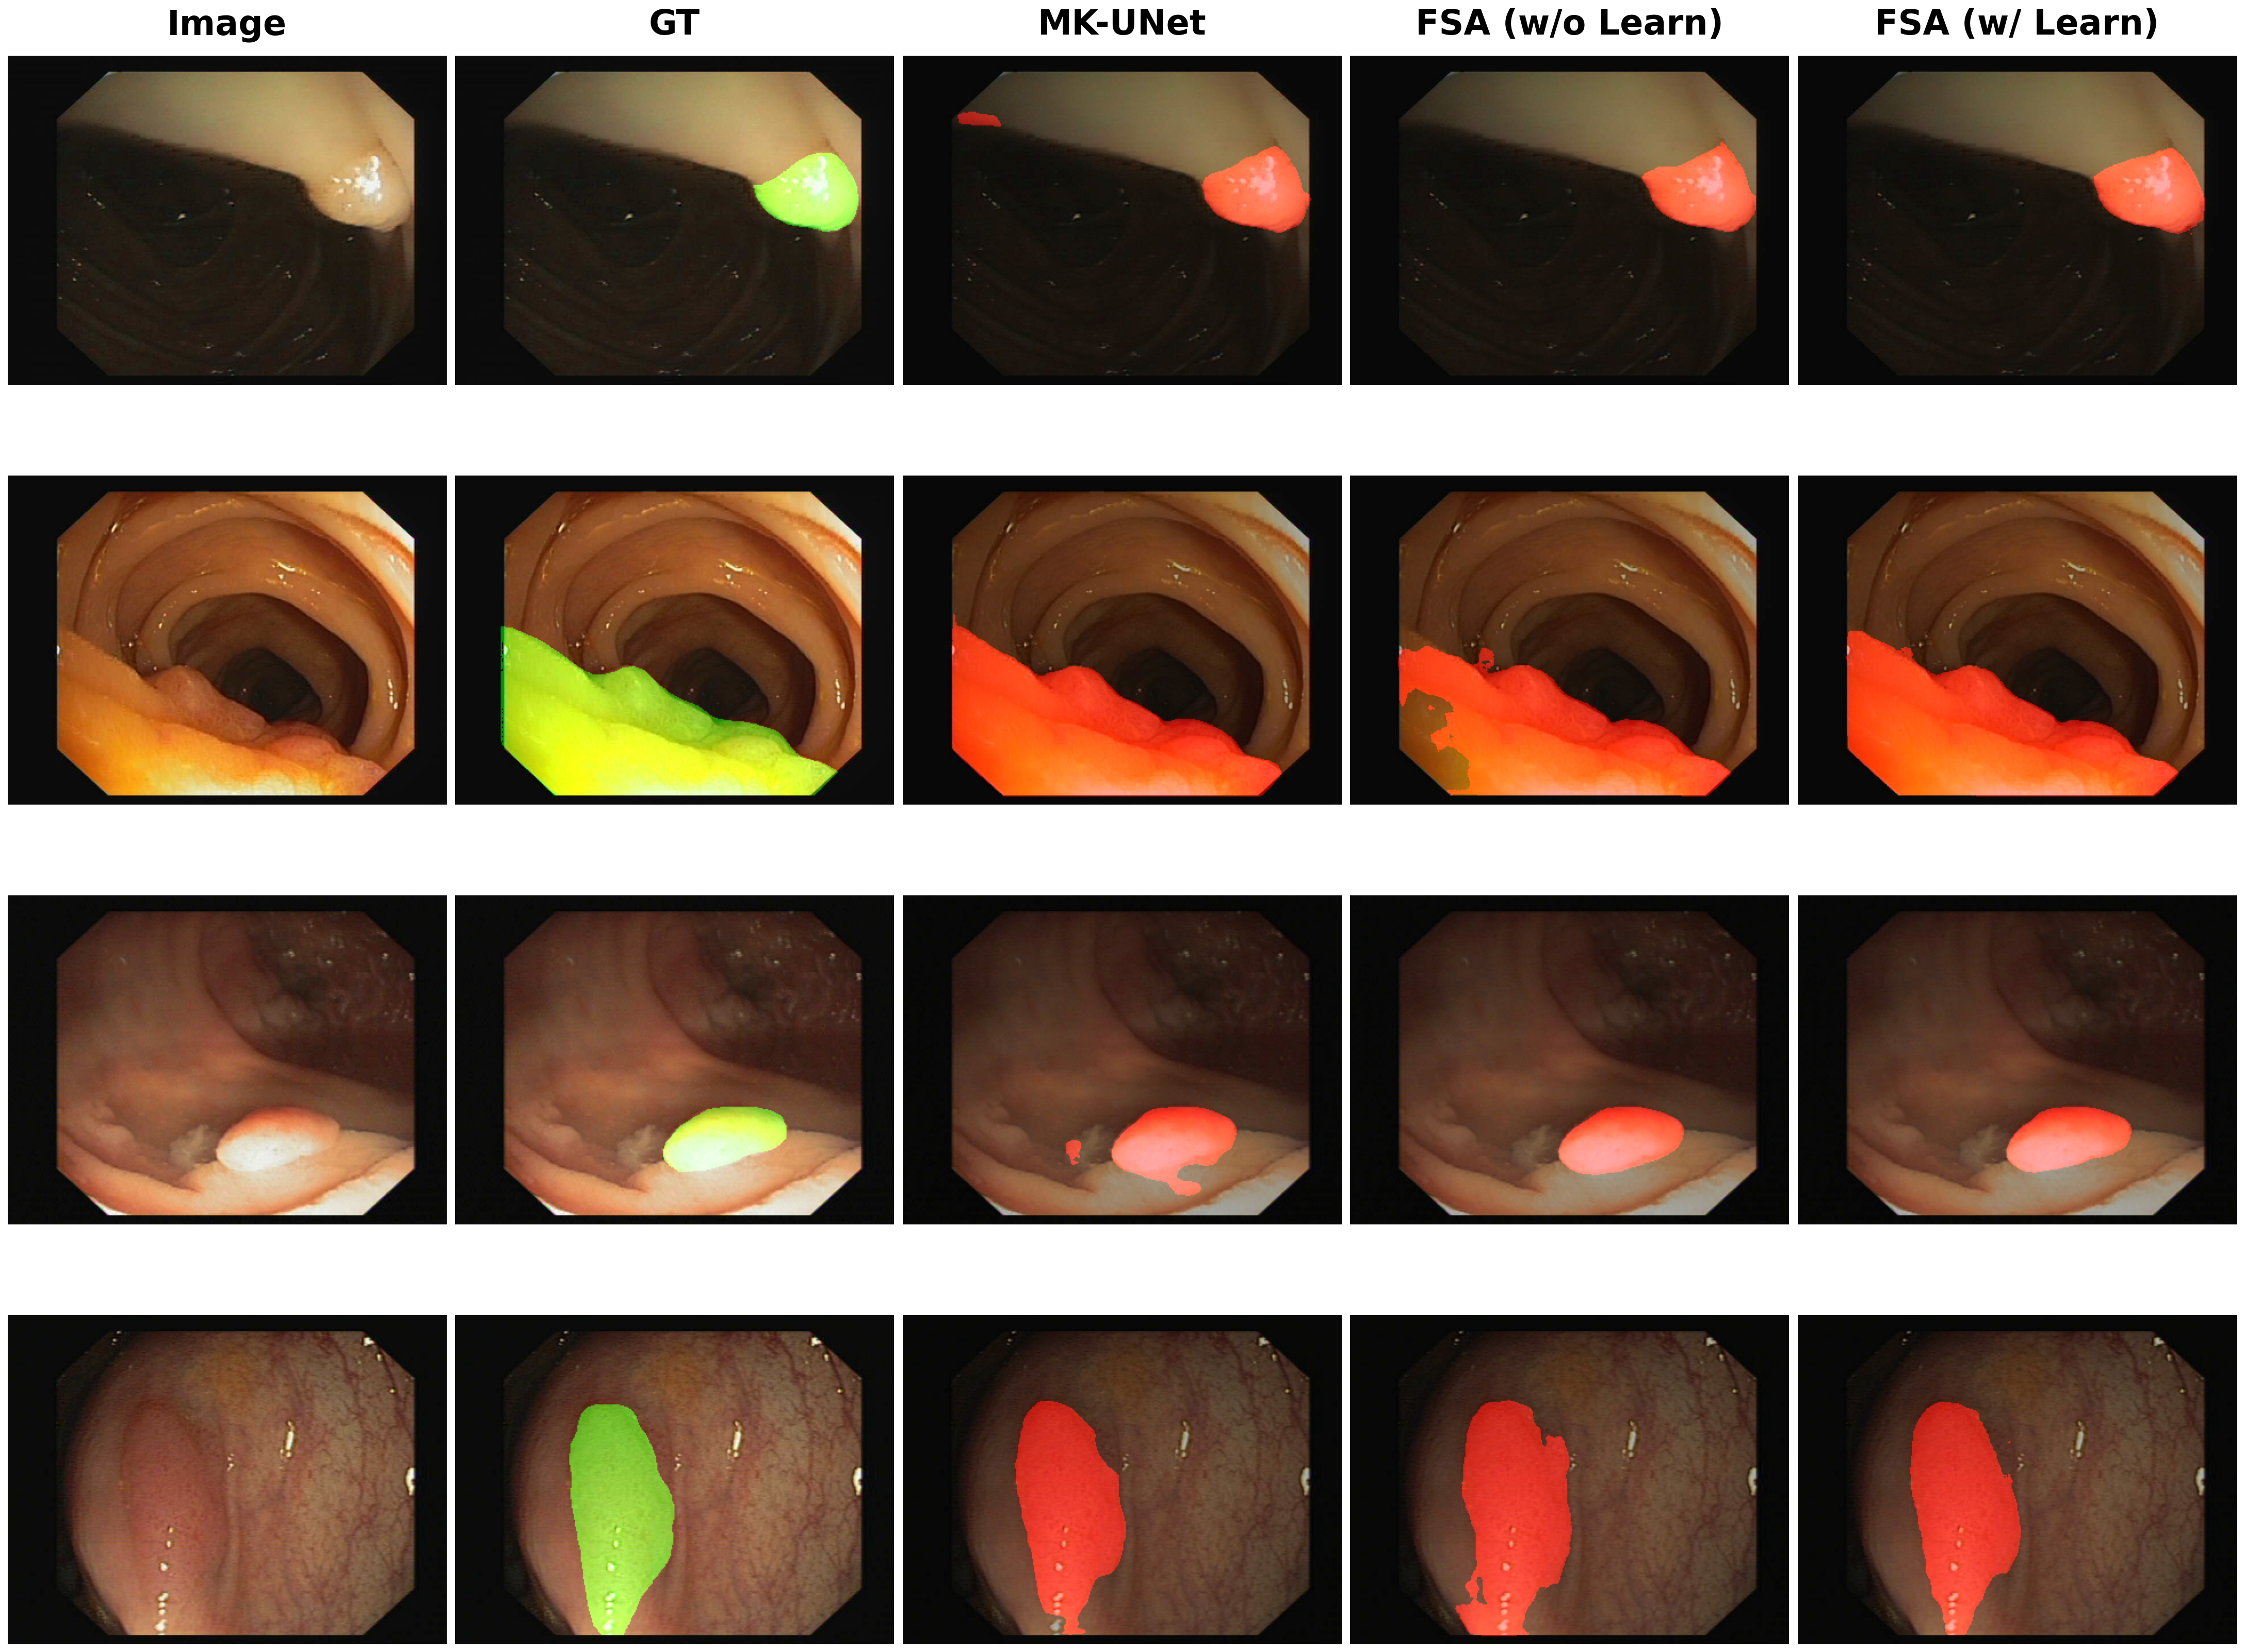
\includegraphics[width=0.9\linewidth]{paper_comparison_figure.png}
    \caption{\chadded{Feature map visualization comparison between the baseline and WCANet (Ours). Compared to the baseline, WCANet exhibits more precise and concentrated attention on the target objects while effectively suppressing background noise.}}
    \label{fig:feature_vis}
\end{figure*}



\subsection{\chadded{\color{blue}Medical Image Segmentation on ClinicDB}}


{\color{blue}

\chadded{\color{blue}To evaluate how WCANet behaves across domains where the frequency characteristics of meaningful features differ substantially from natural ImageNet statistics, we conduct further experiments on medical image segmentation using the ClinicDB dataset. Medical images often exhibit highly unique texture, contrast, and edge distributions compared to natural scenarios. As shown in Table~\ref{tab:clinicdb_domain_adaptation}, directly applying fixed Haar filters provides a marginal improvement over the baseline UNet structure. }

\chadded{\color{blue}In contrast, WCANet equipped with our proposed learnable wavelet filters achieves significant performance gains, reaching 94.41\% Test Dice and 89.69\% Test IoU. This prominent improvement demonstrates that our learnable filters, strictly guided by the orthogonality constraint, can stably and effectively adapt to severe domain and distribution shifts without optimization collapse. The orthogonality constraint ensures that the dynamic multi-band decomposition remains mathematically sound and non-redundant, even when fitting highly specific, non-natural frequency domains.}


\chadded{\color{blue}To intuitively demonstrate the superiority of our proposed WCANet in spatial feature extraction, we visualize the intermediate feature maps of both the baseline model and our WCANet. As shown in Fig.~\ref{fig:feature_vis}, the baseline model tends to capture redundant background information and exhibits scattered, unfocused responses. In contrast, by decoupling feature modeling and employing the Learnable Wavelet Spatial Attention (LWSA), WCANet successfully suppresses irrelevant noise and concentrates its responses much more precisely on the discriminative regions of the target objects. This qualitative comparison provides strong empirical evidence that our Cascade Channel-Spatial Attention (CCSA) mechanism effectively separates redundant features and achieves highly precise spatial modeling.}

}


\subsection{Model Analyses}



In this subsection, we conduct ablation experiments by using WCANet on ImageNet-100, which is a subset of ImageNet-1K. All models are trained under the same settings~\cite{graham2021levit,liu2023efficientvit} with 100 epochs.

\begin{table}[pos=h]
\centering
\caption{\chadded{Ablation study of learnable filters at different stages on WCANet-T1.}}
\label{tab:stage_ablation}
% 稍微缩小一点字号，避免缩放后字体看起来太扁
\small 
% 调整列间距（默认是6pt，改小一点可以让缩放的幅度更小，字号显得更大）
\setlength{\tabcolsep}{4pt} 
\resizebox{\columnwidth}{!}{%
\begin{tabular}{lcccc}
\toprule
\textbf{Configuration} & \textbf{Params (M)} & \textbf{FLOPs (M)} & \textbf{Top-1 Acc (\%)} & \textbf{$\Delta$ (\%)} \\
\midrule
Baseline (None)        & 2.119 & 79.55 & 71.6 & - \\
Stage 0 Only           & 2.122 & 79.55 & 71.9 & +0.3 \\
Stage 1 Only           & 2.129 & 79.55 & 72.6 & +1.0 \\
Stage 2 Only           & 2.138 & 79.55 & 72.6 & +1.0 \\
Stage 0 \& 1           & 2.131 & 79.55 & 72.6 & +1.0 \\
All Stages             & 2.149 & 79.55 & 72.9 & +1.3 \\
\bottomrule
\end{tabular}%
}
\end{table}



\chadded{\textbf{Analysis of Learnable Wavelet Filters.} 
To clearly reveal the individual contribution of learnable filters at different network depths, we conduct ablation studies on WCANet-T1 by enabling learnable wavelet filters in different stages independently. As shown in Table~\ref{tab:stage_ablation}, introducing learnable filters at any single stage (Stage 0, 1, or 2) yields a performance improvement over the baseline (71.6\%), demonstrating the general effectiveness of this design. Notably, the independent contributions of Stage 1 and Stage 2 (both +1.0\%) are significantly greater than that of Stage 0 (+0.3\%). We attribute this to the fact that mid-to-late stages contain more abstract and complex semantic information. In these deeper stages, data-driven learnable filters can more accurately capture high-dimensional frequency distribution differences than fixed Haar filters. In contrast, the early Stage 0 primarily captures basic edges and textures, for which fixed filters already provide a relatively strong foundation. Finally, enabling learnable filters across all stages synergistically achieves the optimal performance of 72.9\% (+1.3\%), confirming the necessity of multi-stage adaptive decomposition.
}




% 消融实验我们使用WCANet-T4在ImageNet-100上进行实验。ImageNet-100是ImageNet-1k的子集。所有模型采用相同的训练设置，每个模型均训练100轮。

 % \textbf{分析可学习小波滤波器的有效性。}


% \begin{table}[t]
% \centering
% \caption{Top-1 accuracy under different configurations of learnable wavelet filters in LWSA across stages. Green indicates fixed wavelet filters; blue indicates learnable wavelet filters.}
% \label{tab:learnable_wt_ablation}
% \begin{tabular}{cccc}
% \toprule
% Stage 0 & Stage 1 & Stage 2 & Top-1 (\%) \\
% \midrule
% \cellcolor{LightGreen}Fixed       & \cellcolor{LightGreen}Fixed      & \cellcolor{LightGreen}Fixed      & 78.4 \\
% \cellcolor{LightBlue}Learnable    & \cellcolor{LightGreen}Fixed      & \cellcolor{LightGreen}Fixed      & 78.9 \\
% \cellcolor{LightBlue}Learnable    & \cellcolor{LightBlue}Learnable   & \cellcolor{LightGreen}Fixed      &  79.7 \\
% \cellcolor{LightBlue}Learnable    & \cellcolor{LightBlue}Learnable   & \cellcolor{LightBlue}Learnable   & \textbf{80.6} \\
% \bottomrule
% \end{tabular}
% \end{table}


\begin{table}[pos=h]
\centering
\caption{Top-1 accuracy under different configurations of learnable wavelet filters in LWSA across stages. Fix indicates fixed wavelet filters; learnable indicates learnable wavelet filters.}
\label{tab:learnable_wt_ablation}
\begin{tabular}{cccc}
\toprule
Stage 0 & Stage 1 & Stage 2 & Top-1 (\%) \\
\midrule
Fixed       & Fixed      & Fixed      & 78.4 \\
Learnable    & Fixed      & Fixed      & 78.9 \\
Learnable    & Learnable   & Fixed      &  79.7 \\
Learnable    & Learnable   & Learnable   & \textbf{80.6} \\
\bottomrule
\end{tabular}
\end{table}


\textbf{Analysis of Learnable Wavelet Filters.} To investigate the effectiveness of learnable wavelet filters in LWSA, we conduct ablation studies by progressively enabling filter learning across stages. As shown in Table~\ref{tab:learnable_wt_ablation}, when all stages use fixed wavelet filters, the model achieves a baseline Top-1 accuracy of 78.4\%. Introducing learnable filters in Stage 0 alone improves performance to 78.9\%, demonstrating that data-adaptive decomposition enhances spatial feature modeling even at early layers. Finally, when all stages employ learnable wavelet filters, the model achieves the highest accuracy of 80.6\%, confirming that end-to-end trainable filters consistently improve feature modeling ability. This trend clearly indicates that learning wavelet bases from data, rather than relying on handcrafted ones, leads to more effective feature separation and reconstruction.




\begin{table}[pos=h]
\centering
\caption{LWSA and others.}
\label{tab:ablation_lwsa_attention}
  \begin{tabular}{lcc}
\toprule
Strategy & FLOPs & Top-1 \\
\midrule
Identity & 313 & 75.2 \\
$7\times7$ DW & 318 & 79.1 \\
LS Conv  & 321 & 80.4 \\
\rowcolor[gray]{0.92}
\textbf{LWSA} & 313 & \textbf{80.6} \\
\bottomrule
\end{tabular}
\end{table}


\begin{table}[pos=h]
\centering
  \caption{HH sub-hand method} 
  \label{tab:HH_method}
  \centering
  \begin{tabular}{lcc}
\toprule
Strategy & FLOPs & Top-1\\
\midrule
ALL DW & 318 & 79.1 \\
HH Identity & 316 & 79.0 \\
\bottomrule
\end{tabular}
\end{table}

\textbf{Analysis of Wavelet Spatial Attention.} To verify the rationality of the Wavelet Spatial Attention (WSA) design proposed in LWSA, we compare LWSA with other feature extraction methods. We design three approaches: the first one directly applies an identity transformation to the LL, LH, and HL sub-bands; the second one performs 7x7 depthwise convolution on each of the three sub-bands; and the third one is our proposed WSA. As shown in Tab. \ref{tab:ablation_lwsa_attention}, LWSA achieved a top-1 accuracy of up to 80.6\% while having fewer FLOPs than \chadded{\color{blue}both} the 7x7 depthwise convolution \chadded{ \color{blue} and the LS Conv} method. To verify whether the HH sub-band is beneficial to model performance, we conducted experiments by convolving all sub-bands and only convolving the LL, HL, and LH sub-bands. As shown in Tab.\ref{tab:HH_method}, the result indicates that neglecting to perform convolution on the HH sub-band leads to lower FLOPs without significant changes in top-1 accuracy, validating the effectiveness of the feature separation method proposed in LWSA.






\begin{table} [pos=h]
    \centering
    \caption{All variants are based on WCANet-T4 and evaluated on ImageNet-100 with 100 training epochs.}
    \begin{tabular}{c|c|c}
    \toprule
     Function &  \makecell{60 Epoch \\ Top1-Acc(\%)} & \makecell{100 Epoch \\ Top1-Acc(\%)}  \\
     \midrule
        $HL$ & 73.01\% & 78.04\% \\
        $HH$ & 73.16\% & 77.92\% \\
        $LL$ & 71.92\% & 77.31\% \\ \midrule
        $HL \odot LH$ &  77.58\% & 80.57\% \\
        $HH \odot LH$ &  76.71\% & 80.64\% \\
        $HL \odot HH$ &  76.64\% & 80.61\% \\ \midrule
        $HL \odot LH \odot HH$ & 76.21\% & 80.54\%  \\
    \bottomrule
    \end{tabular}
    \label{tab:placeholder}
\end{table}



\textbf{Analyze the effectiveness of different feature weight generation methods.} We evaluated the impact on model performance when feature weights are generated from one, two, or three subbands. 
The experimental results are shown in Table~\ref{tab:placeholder}. It can be observed that feature weights derived from a single subband yield the lowest Top-1 accuracy, whereas those generated from two or three subbands achieve better performance.
However, compared to other approaches, the $HL \odot LH$ variant demonstrates superior convergence over variants using three or other combinations of subbands. This strongly validates the effectiveness of the $HL \odot LH$ method.

% 分析不同特征权重的有效性。我们试验了由单个、两个、或三个子带生成的特征权重对于模型的性能影响。实验结果如表\ref{tab:placeholder}所示，
% 可以看出单个子带生成的特征权重的最终Top-1%最低，而由两子带或三个子带生成的特征权重表现出更好的性能。
% 但是相比较其他方法，$HL \odot LH$变体的收敛优于由三种或其他子带生成的特征权重变体。这充分验证了$HL \odot LH$方法的有效性。







\begin{table}[pos=h]
\centering
\caption{\chadded{Ablation study of individual components (ESE and LWSA) within the CCSA block.}}
\label{tab:component_ablation}
\begin{tabular}{lc}
\toprule
\textbf{Configuration} & \textbf{Top-1 Acc (\%)} \\
\midrule
Baseline (None)     & 80.2 \\
ESE Only            & 82.7 \\
LWSA Only           & 83.3 \\
\rowcolor[gray]{0.92}
CCSA (ESE + LWSA)   & \textbf{85.5} \\
\bottomrule
\end{tabular}
\end{table}




\chadded{\textbf{Ablation Study of CCSA Components.} 
To isolate and quantify the individual contributions of the ESE module and the Learnable Wavelet Spatial Attention (LWSA), we conduct a component-wise ablation study on the CCSA block. As shown in Table~\ref{tab:component_ablation}, both components independently improve model performance. Compared to the baseline model (80.2\%), introducing only the ESE module or only the LWSA module yields significant improvements of +2.5\% and +3.1\%, respectively. The slightly better independent performance of LWSA (83.3\%) over ESE (82.7\%) indicates that our wavelet-based spatial attention plays a particularly crucial role in visual feature extraction. Furthermore, combining ESE and LWSA into the complete cascaded CCSA block achieves the highest Top-1 accuracy (85.5\%). This confirms that channel-wise and spatial-level feature enhancements are highly complementary, and the cascaded design is strictly necessary for comprehensive and effective feature extraction.
}







\begin{table}[pos=h]
    \color{blue}
    \centering
    \caption{\textcolor{blue}{\textit{\chadded{Ablation study of filter types on COCO object detection (RetinaNet 1x schedule).}}}}
    \label{tab:coco_filter_ablation}
    % 稍微缩小列间距，避免 resizebox 将字体缩得太小
    \setlength{\tabcolsep}{3pt}
    % 强制将表格限制在单栏宽度（\columnwidth）内
    \resizebox{\columnwidth}{!}{%
    \begin{tabular}{lcccccc}
    \toprule
    \textbf{Filter Type} & \textbf{AP} & \textbf{AP$_{50}$} & \textbf{AP$_{75}$} & \textbf{AP$_S$} & \textbf{AP$_M$} & \textbf{AP$_L$} \\
    \midrule
    Fixed Haar Filters  & 37.8 & 58.2 & 40.2 & 21.3 & 40.9 & 51.0 \\
    Learnable Filters (Ours) & \textbf{38.6} & \textbf{59.0} & \textbf{41.1} & \textbf{22.5} & \textbf{41.5} & \textbf{51.7} \\
    \midrule
    \textit{Degradation ($\Delta$)} & \textit{-0.8} & \textit{-0.8} & \textit{-0.9} & \textit{-1.2} & \textit{-0.6} & \textit{-0.7} \\
    \bottomrule
    \end{tabular}%
    }
\end{table}

\textcolor{blue}{\textit{\chadded{\textbf{Impact of Learnable Filters on Downstream Tasks.} To further validate the effectiveness of our learnable wavelet filters in dense prediction, we conducted an ablation study on the COCO dataset using the RetinaNet framework by replacing the learnable filters with fixed Haar filters. As shown in Table~\ref{tab:coco_filter_ablation}, reverting to fixed filters leads to a noticeable degradation in overall performance (AP drops by 0.8\%). Notably, the accuracy degradation differs across object categories. The most severe drop occurs in small objects ($AP_S$ decreases by 1.2\%), followed by large objects (-0.7\%) and medium objects (-0.6\%). This scale-aware degradation strongly indicates that data-driven learnable filters are particularly crucial for adaptively distinguishing fine-grained details and subtle edges from background noise, an adaptability that rigid fixed filters fail to provide.}}}





\section{Conclusion}

% 现有的基于CNN的轻量级网络

In this work, we propose WCANet, a lightweight neural network that achieves efficient feature modeling at a low computational cost. The core of WCANet is the Cascade Channel-Spatial Attention module (CCSA).  CCSA decomposes feature extraction into the channel-wise and spatial levels. In the channel-wise, CCSA employs the ESE Module to augment key feature channels. In the spatial dimension, CCSA employs Learnable Wavelet Spatial Attention (LWSA) to achieve efficient and effective spatial modeling. CCSA enables WCANet to better focus on key features under low computational cost. WCANet achieves state-of-the-art speed-accuracy trade-offs on multiple devices.







\begin{figure}[pos=t]
    \centering
    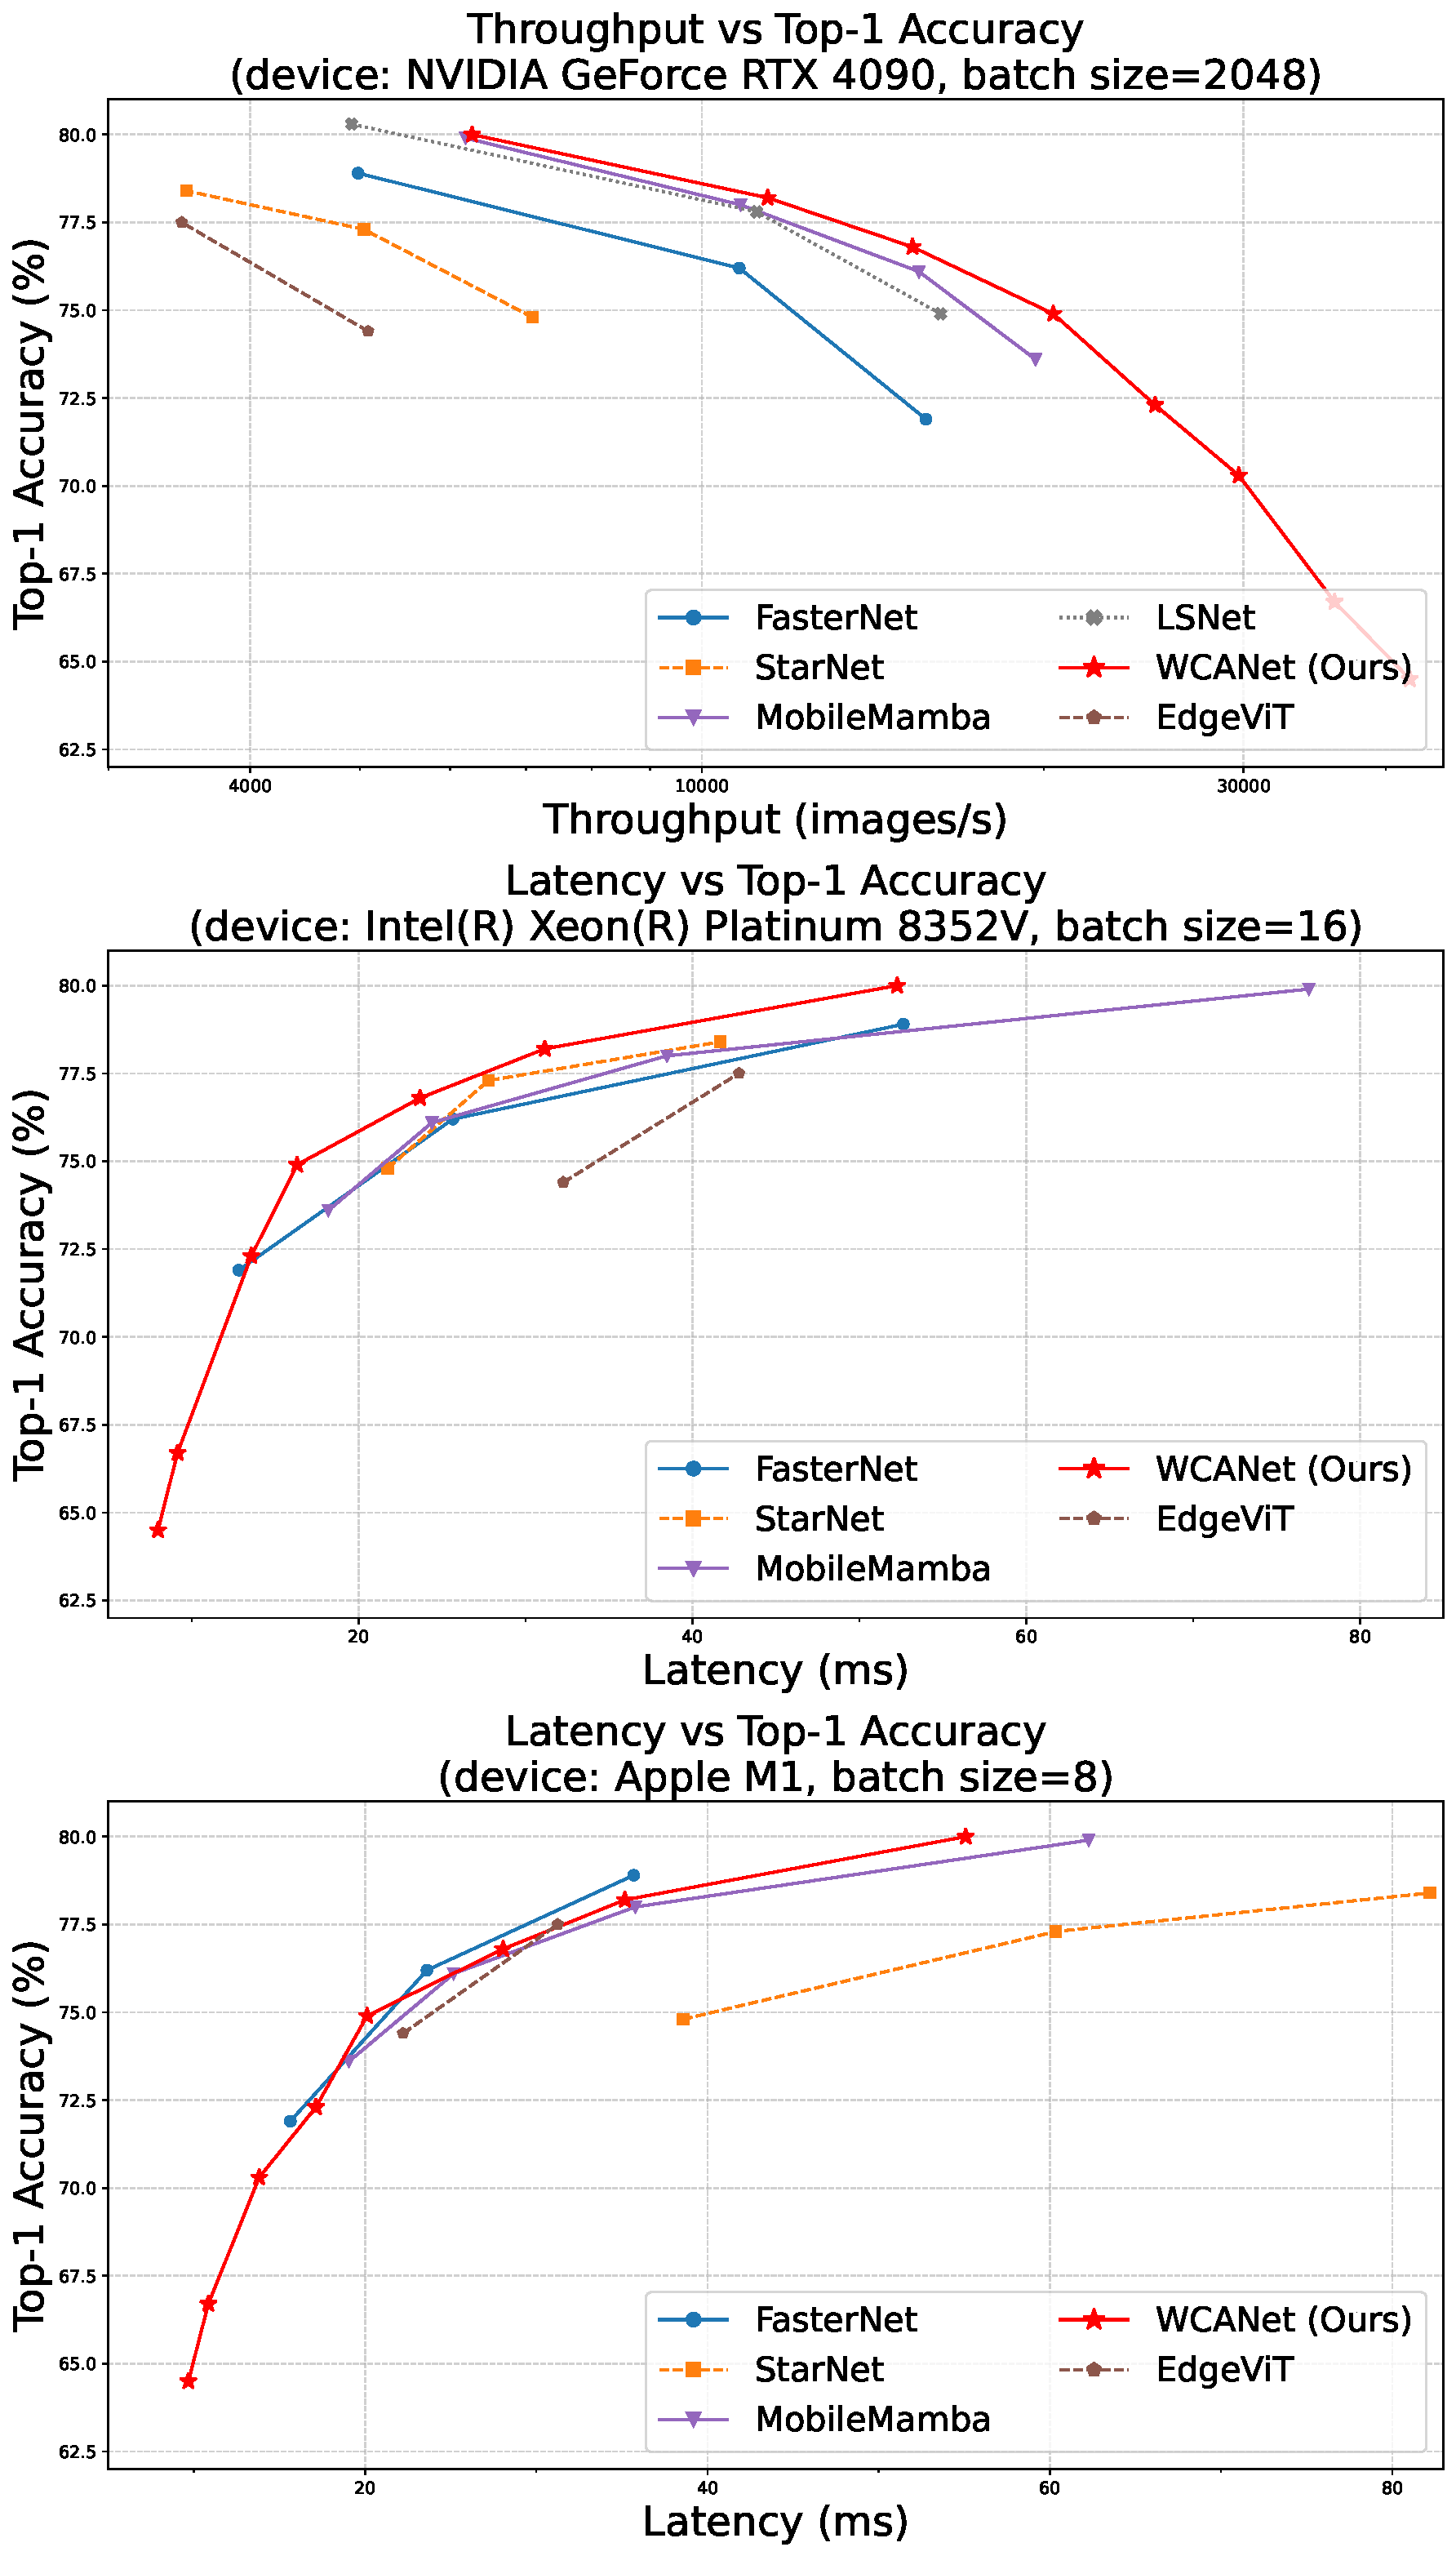
\includegraphics[width=1.\linewidth]{combined_gpu_cpu_m1_performance.pdf}
    \caption{WCANet most efficiently balances accuracy–throughput and accuracy–latency trade-offs across devices.}
    \label{fig:GPU_throught}
\end{figure}










































\appendix
\section{Appendix}


\begin{figure*} 
    \centering
    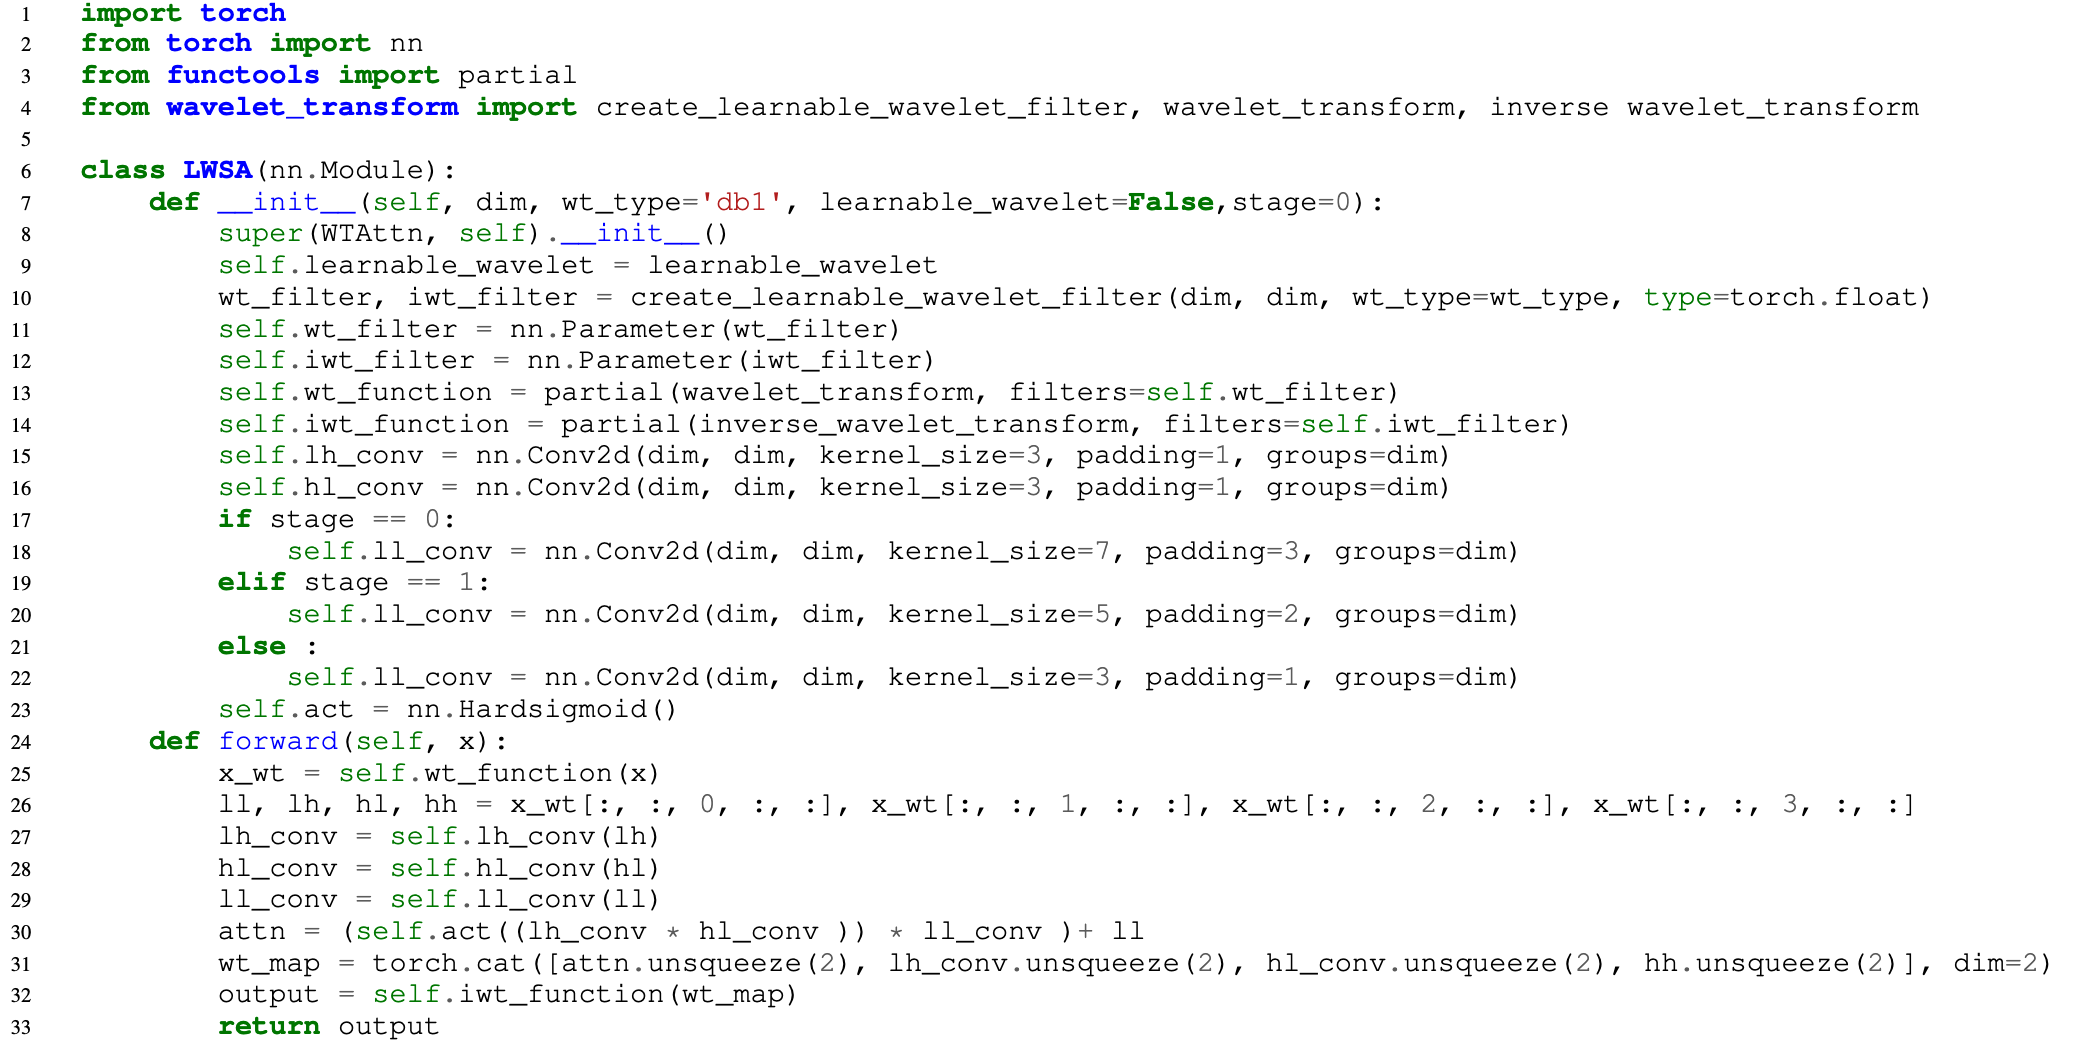
\includegraphics[width=0.9\linewidth]{code.png}
    \caption{The Pytorch code of LWSA. Due to space limitations, the specific implementation method of creating learnable wavelet filters is not shown.}
    \label{listing:code}
\end{figure*}

In this appendix, we provide more details on the experimental setup, architecture configuration, implementation of LWSA, limitations, and future work.

\subsection{ImageNet-1k experimental settings}


For the image classification task on ImageNet-1k, our training scheme is shown in Tab.\ref{tab:train_detail}. Since the maximum downsampling of WCANet is $\times128$, we use an image size of $256\times256$ for both training and testing. We found that T6 and T8 did not reach the highest accuracy at 300 rounds, so the training epochs for T6 and T8 are 400 epochs. We use the AdamW optimizer in combination with a cosine learning rate scheduler. The initial learning rate is set to $3\times10^{-3}$, and the total batch size is set to 1024. For data augmentation, we utilized methods such as Mixup, CutMix, and Random Erasing. We also use EMA to enhance the stability of training. \chadded{Furthermore, to ensure a smooth startup and prevent gradient instability during the early stages of training, we consistently employ a linear warmup strategy (e.g., 20 epochs for ImageNet-1k) before the cosine learning rate decay.}

\begin{table}
\centering
\caption{Training Details on ImageNet}
\label{tab:train_detail}
\begin{tabular}{l|ccccc}
\hline
Variants & \multicolumn{3}{|c}{T1, T2, T2d5, T3, T4, T5} & T6 & T8\\
\hline
Train Res          & \multicolumn{5}{c}{256}                                    \\
Test Res           & \multicolumn{5}{c}{256}                                    \\ \midrule
Epochs          & \multicolumn{3}{c}{300}   & \multicolumn{2}{|c}{400} \\ \midrule
Batch size &   \multicolumn{5}{c}{1024}  \\ 
Optimizer & \multicolumn{5}{c}{AdamW}  \\
Momentum & \multicolumn{5}{c}{0.9/0.999} \\
LR & \multicolumn{5}{c}{3e-4} \\
LR decay  & \multicolumn{5}{c}{cosine} \\
Warmup epochs & \multicolumn{5}{c}{20} \\
Warmup schedule & \multicolumn{5}{c}{linear} \\ \midrule
 Label Smooth & \multicolumn{5}{c}{0.1} \\
 Mixup           & \multicolumn{5}{c}{0.8}     \\
 Cutmix          & \multicolumn{5}{c}{1.0}     \\ 
  Random Erasing & \multicolumn{5}{c}{0.25} \\ \midrule
Dropout  & \multicolumn{4}{c|}{\ding{55}} & 0.01  \\ \midrule
  EMA & \multicolumn{5}{c}{\ding{51}} \\
  \midrule


% 后续行可在此添加，例如：模型配置、学习率、epoch等
\end{tabular}
\end{table}




\subsection{Architectural Details}

\chadded{\color{blue}As WCANet incorporates wavelet transform mechanisms across multiple stages, the maximum downsampling factor of the network reaches 128. To ensure the complete alignment of feature dimensions and preserve the structural integrity of the wavelet decomposition, the input resolution must be perfectly divisible by this factor. Therefore, an input resolution of $256 \times 256$ is chosen as an intrinsic architectural requirement, avoiding the extensive feature padding, unnecessary computational overhead, and boundary artifacts that would inevitably arise from using a standard $224 \times 224$ resolution.}

Tab.\ref{tab:achitecture} presents the architectural details of the three-stage WCANet variants, and Tab.\ref{tab:achitecture_T8} shows the details of the four-stage WCANet variants.

\begin{table}
    \caption{Architectural details of WCANet-T1, WCANet-T3, and WCANet-T5.}
    \label{tab:achitecture}
    \small
    \centering
    \resizebox{\columnwidth}{!}{%
    \begin{tabular}{c|c|c|c|c|c|c}
    \toprule
    \multirow{2}{*}{Stage} & \multirow{2}{*}{Resolution} &    \multirow{2}{*}{Type} & \multirow{2}{*}{Config} & \multicolumn{3}{c}{WCANet}  \\ \cline{5-7}
    & & & & T1 & T3 & T5 \\
    \hline
    \hline
    \multirow{8}{*}{stem} & \multirow{2}{*}{$\frac{H}{2} \times \frac{W}{2}$} & \multirow{2}{*}{Convolution} & \multirow{2}{*}{channels} & \multirow{2}{*}{8} & \multirow{2}{*}{13} & \multirow{2}{*}{16} \\
    & & & & & \\
    \cline{2-7}
    & \multirow{2}{*}{$\frac{H}{4} \times \frac{W}{4}$} & \multirow{2}{*}{Convolution} & \multirow{2}{*}{channels} & \multirow{2}{*}{16} & \multirow{2}{*}{26} & \multirow{2}{*}{32} \\
    & & & & & \\
    \cline{2-7}
    & \multirow{2}{*}{$\frac{H}{8} \times \frac{W}{8}$} & \multirow{2}{*}{Convolution} & \multirow{2}{*}{channels} & \multirow{2}{*}{32} & \multirow{2}{*}{52} & \multirow{2}{*}{64} \\
    & & & & & \\
    \cline{2-7}
     & \multirow{2}{*}{$\frac{H}{8} \times \frac{W}{8}$} & \multirow{2}{*}{Convolution} & \multirow{2}{*}{channels} & \multirow{2}{*}{64} & \multirow{2}{*}{104} & \multirow{2}{*}{128} \\
    & &  &  &  &  \\
    \hline

    \multirow{2}{*}{1} & \multirow{2}{*}{$\frac{H}{16} \times \frac{W}{16}$} & \multirow{2}{*}{CCSA Block} & channels & 64 & 104 & 128 \\
    \cline{4-7}
    & & & blocks & 2 & 2 & 3 \\
    \hline
    \multirow{2}{*}{2} & \multirow{2}{*}{$\frac{H}{32} \times \frac{W}{32}$} & \multirow{2}{*}{CCSA Block} & channels & 128 & 208 & 256 \\
    \cline{4-7}
    & &  & blocks & 3 & 3 & 4 \\
    \hline
    \multirow{2}{*}{3} & \multirow{2}{*}{$\frac{H}{64} \times \frac{W}{64}$} & \multirow{2}{*}{CCSA Block} & channels & 256 & 416 & 512 \\
    \cline{4-7}
    & & & blocks & 2 & 2 & 3 \\
    \bottomrule
    \end{tabular}
    }
    \vspace{-10pt}
\end{table}

\begin{table} [pos=t]
    \caption{Architectural details of WCANet-T8.}
    \label{tab:achitecture_T8}
    \small
    \centering
    \resizebox{\columnwidth}{!}{%
    \begin{tabular}{c|c|c|c|c}
    \toprule
    \multirow{2}{*}{Stage} & \multirow{2}{*}{Resolution} &    \multirow{2}{*}{Type} & \multirow{2}{*}{Config} & \multirow{2}{*}{WCANet-T8}  \\ 
    & & & & \\
    \hline

    \hline
    \multirow{6}{*}{stem} & \multirow{2}{*}{$\frac{H}{2} \times \frac{W}{2}$} & \multirow{2}{*}{Convolution} & \multirow{2}{*}{channels} & \multirow{2}{*}{24} \\
    & & & & \\
    \cline{2-5}
     & \multirow{2}{*}{$\frac{H}{4} \times \frac{W}{4}$} & \multirow{2}{*}{Convolution} & \multirow{2}{*}{channels} & \multirow{2}{*}{48} \\
    & & & & \\
    \cline{2-5}
    & \multirow{2}{*}{$\frac{H}{8} \times \frac{W}{8}$} & \multirow{2}{*}{Convolution} & \multirow{2}{*}{channels} & \multirow{2}{*}{96} \\
    & & & & \\
    \hline
    \multirow{2}{*}{1} & \multirow{2}{*}{$\frac{H}{8} \times \frac{W}{8}$} & \multirow{2}{*}{CCSA Block} & channels & 96  \\
    \cline{4-5}
    & & & blocks & 2 \\
    \hline
    \multirow{2}{*}{2} & \multirow{2}{*}{$\frac{H}{16} \times \frac{W}{16}$} & \multirow{2}{*}{CCSA Block} & channels & 192 \\
    \cline{4-5}
    & & & blocks & 3 \\
    \hline
    \multirow{2}{*}{3} & \multirow{2}{*}{$\frac{H}{32} \times \frac{W}{32}$} & \multirow{2}{*}{CCSA Block} & channels & 384 \\
    \cline{4-5}
    & & & blocks & 4 \\
    \hline
    \multirow{2}{*}{4} & \multirow{2}{*}{$\frac{H}{64} \times \frac{W}{64}$} & \multirow{2}{*}{CCSA Block} & channels & 640 \\
    \cline{4-5}
    & & & blocks & 5 \\
    \bottomrule
    \end{tabular}
    }
    \vspace{-10pt}
\end{table}


% \begin{figure*} 
%     \centering
%     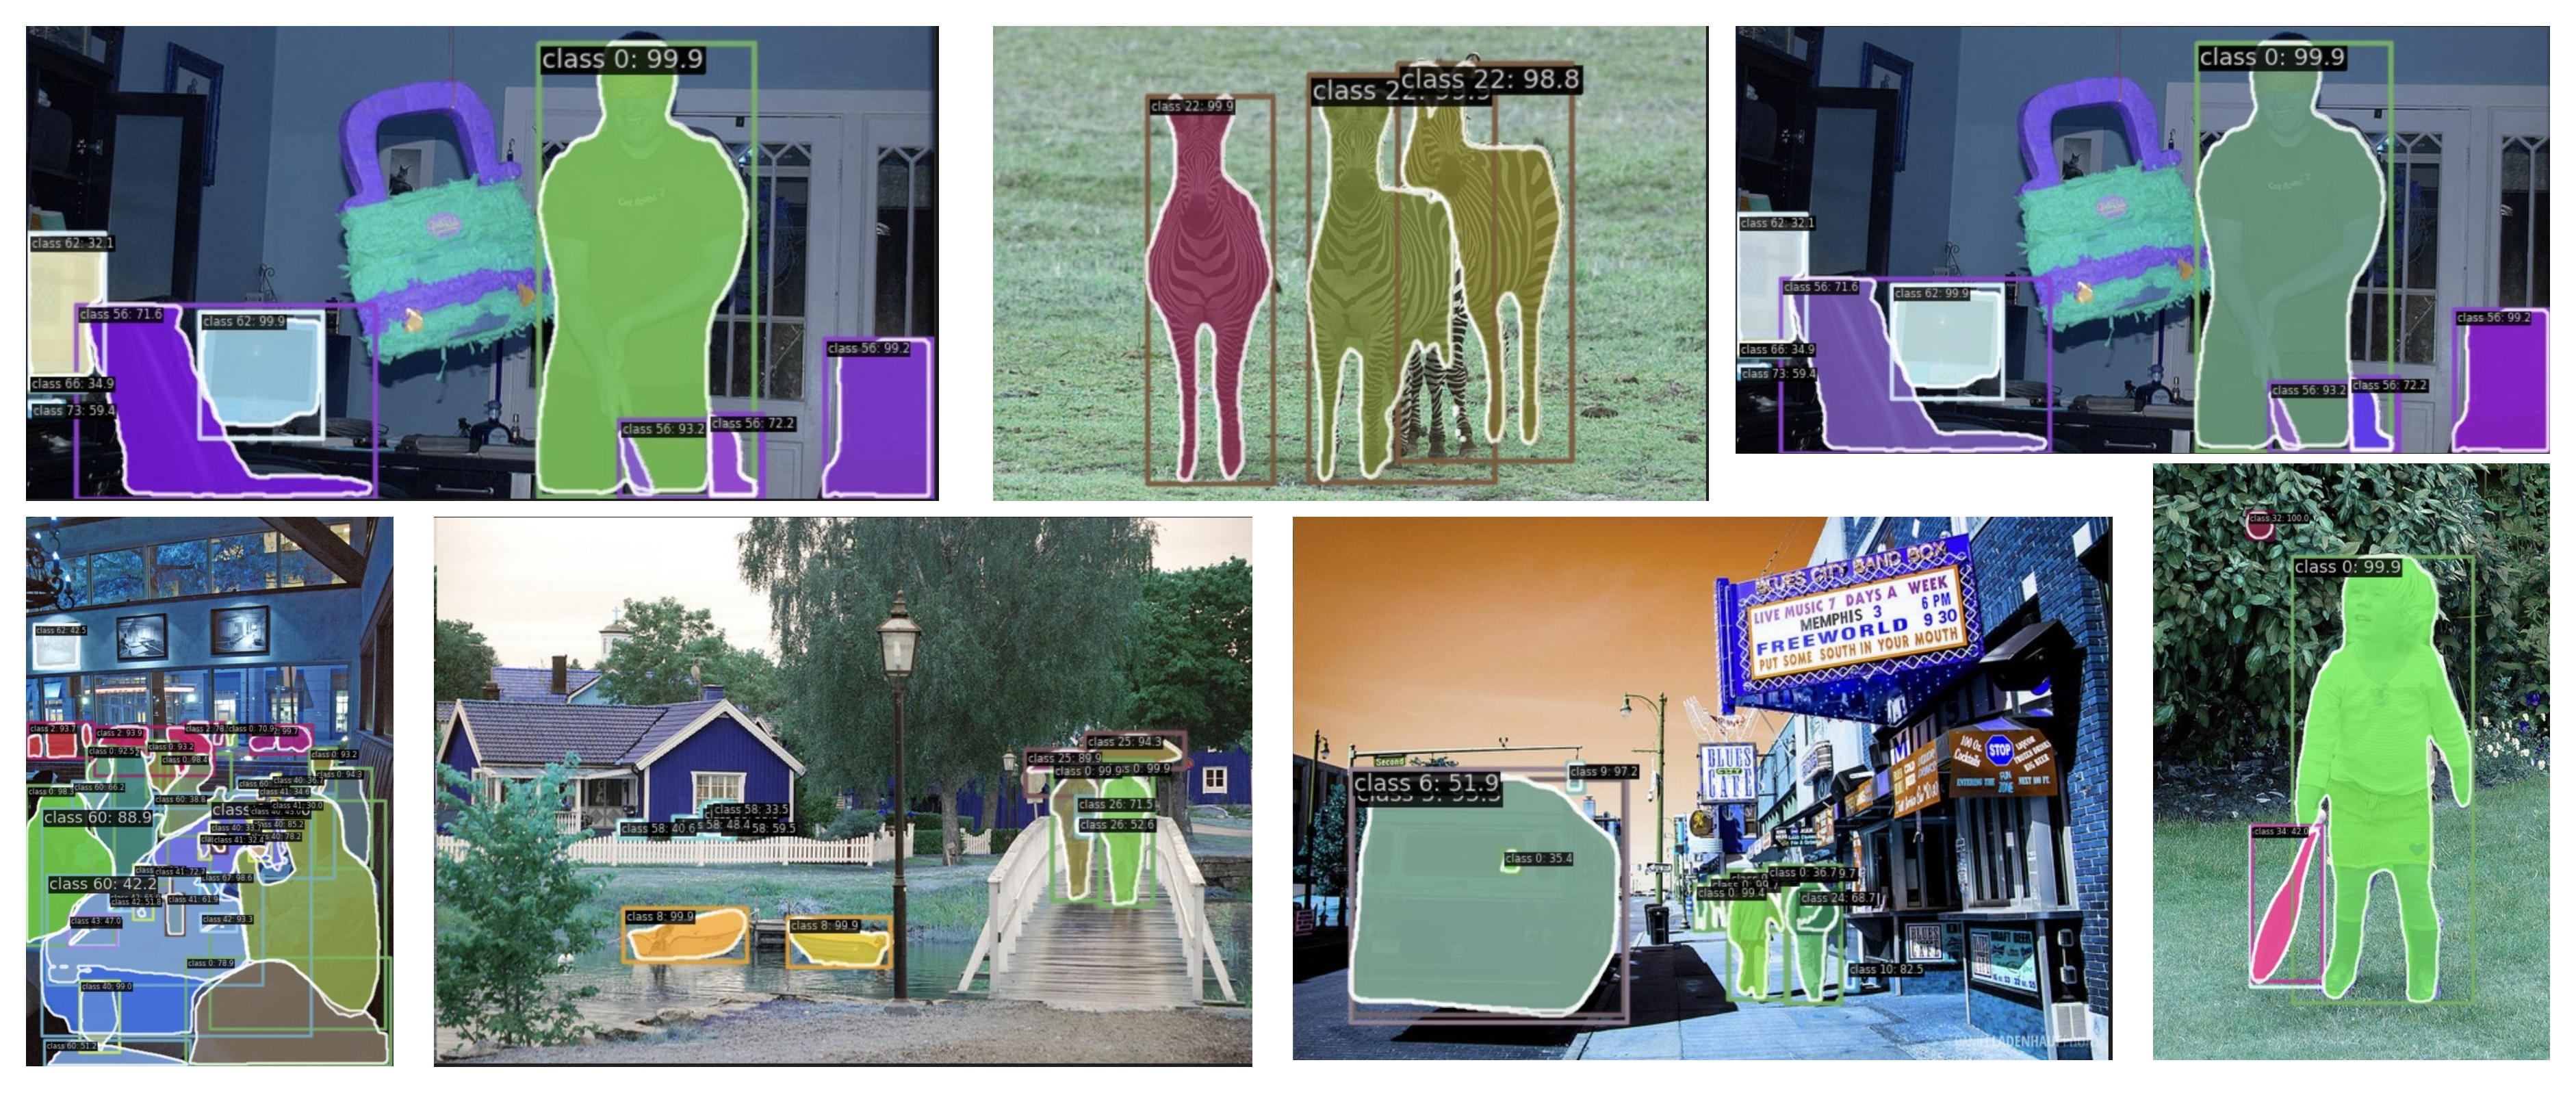
\includegraphics[width=0.9\linewidth]{visualization.pdf}
%     \caption{Qualitative results for object detection and instance segmentation on COCO-2017.}
%     \label{fig:COCO_vis}
% \end{figure*}








\subsection{The code of LWSA}


To present the implementation of LWSA more intuitively, we provide the PyTorch code for LWSA. The specific code is shown in Listing~\ref{listing:code}. Due to space limitations, some functions are not fully displayed.




% \begin{minted}{c}
% int main() {
% printf("hello, world");
% return 0;
% }
% \end{minted}





\subsection{Limitation and Future Work}


{ \color{blue}
\textbf{Limitation.} While WCANet achieves a favorable speed-accuracy trade-off, our current evaluation focuses on GPU and CPU platforms, with dedicated mobile hardware deployment remaining a primary next step. Additionally, the current stage-dependent kernel size schedule ($k=7, 5, 3$) is fixed, which may not optimally adapt to the varying spatial frequency distributions across highly diverse visual tasks. Finally, as a pure CNN, our model's performance in complex downstream dense prediction tasks still lags slightly behind the latest ViT and SSM-based frameworks.

\textbf{Future Work.} We will validate the model's efficiency on edge devices and publish the results on GitHub. To further bridge the performance gap in downstream tasks, we will explore architectural fusion strategies that integrate WCANet with other paradigms without increasing the computational burden. Furthermore, we intend to investigate dynamic, multi-perspective feature learning strategies, drawing inspiration from recent advancements such as HMPFormer~\cite{usman2025hmpformer}, to enhance the model's architectural flexibility and generalization capability.

}








\printcredits

% %% Loading bibliography style file
% %\bibliographystyle{model1-num-names}
% \bibliographystyle{unsrt}

% \bibliographystyle{unsrt}

% % Loading bibliography database
% \bibliography{cas-refs}




\begin{thebibliography}{10}

\bibitem{han2022survey}
Kai Han, Yunhe Wang, Hanting Chen, Xinghao Chen, Jianyuan Guo, Zhenhua Liu, Yehui Tang, An~Xiao, Chunjing Xu, Yixing Xu, et~al.
\newblock A survey on vision transformer.
\newblock {\em IEEE transactions on pattern analysis and machine intelligence}, 45(1):87--110, 2022.

\bibitem{he2016deep}
Kaiming He, Xiangyu Zhang, Shaoqing Ren, and Jian Sun.
\newblock Deep residual learning for image recognition.
\newblock In {\em Proceedings of the IEEE conference on computer vision and pattern recognition}, pages 770--778, 2016.

\bibitem{dosovitskiy2020image}
Alexey Dosovitskiy.
\newblock An image is worth 16x16 words: Transformers for image recognition at scale.
\newblock {\em arXiv preprint arXiv:2010.11929}, 2020.

\bibitem{liu2022convnet}
Zhuang Liu, Hanzi Mao, Chao-Yuan Wu, Christoph Feichtenhofer, Trevor Darrell, and Saining Xie.
\newblock A convnet for the 2020s.
\newblock In {\em Proceedings of the IEEE/CVF conference on computer vision and pattern recognition}, pages 11976--11986, 2022.

\bibitem{liu2021swin}
Ze~Liu, Yutong Lin, Yue Cao, Han Hu, Yixuan Wei, Zheng Zhang, Stephen Lin, and Baining Guo.
\newblock Swin transformer: Hierarchical vision transformer using shifted windows.
\newblock In {\em Proceedings of the IEEE/CVF international conference on computer vision}, pages 10012--10022, 2021.

\bibitem{zhang2024vision}
Qiming Zhang, Jing Zhang, Yufei Xu, and Dacheng Tao.
\newblock Vision transformer with quadrangle attention.
\newblock {\em IEEE Transactions on Pattern Analysis and Machine Intelligence}, 46(5):3608--3624, 2024.

\bibitem{li2022efficientformer}
Yanyu Li, Geng Yuan, Yang Wen, Ju~Hu, Georgios Evangelidis, Sergey Tulyakov, Yanzhi Wang, and Jian Ren.
\newblock Efficientformer: Vision transformers at mobilenet speed.
\newblock {\em Advances in Neural Information Processing Systems}, 35:12934--12949, 2022.

\bibitem{maaz2022edgenext}
Muhammad Maaz, Abdelrahman Shaker, Hisham Cholakkal, Salman Khan, Syed~Waqas Zamir, Rao~Muhammad Anwer, and Fahad Shahbaz~Khan.
\newblock Edgenext: efficiently amalgamated cnn-transformer architecture for mobile vision applications.
\newblock In {\em European conference on computer vision}, pages 3--20. Springer, 2022.

\bibitem{liu2023efficientvit}
Xinyu Liu, Houwen Peng, Ningxin Zheng, Yuqing Yang, Han Hu, and Yixuan Yuan.
\newblock Efficientvit: Memory efficient vision transformer with cascaded group attention.
\newblock In {\em Proceedings of the IEEE/CVF conference on computer vision and pattern recognition}, pages 14420--14430, 2023.

\bibitem{mehta2021mobilevit}
Sachin Mehta and Mohammad Rastegari.
\newblock Mobilevit: light-weight, general-purpose, and mobile-friendly vision transformer.
\newblock {\em arXiv preprint arXiv:2110.02178}, 2021.

\bibitem{wadekar2022mobilevitv3}
Shakti~N Wadekar and Abhishek Chaurasia.
\newblock Mobilevitv3: Mobile-friendly vision transformer with simple and effective fusion of local, global and input features.
\newblock {\em arXiv preprint arXiv:2209.15159}, 2022.

\bibitem{yun2024shvit}
Seokju Yun and Youngmin Ro.
\newblock Shvit: Single-head vision transformer with memory efficient macro design.
\newblock In {\em Proceedings of the IEEE/CVF Conference on Computer Vision and Pattern Recognition}, pages 5756--5767, 2024.

\bibitem{khan2025optimal}
Habib Khan, Samee Ullah Khan, Waseem Ullah, and Sung Wook Baik.
\newblock Optimal features driven hybrid attention network for effective video summarization.
\newblock {\em Engineering Applications of Artificial Intelligence}, 158:111211, 2025.



\bibitem{fu2022hungry}
Daniel~Y Fu, Tri Dao, Khaled~K Saab, Armin~W Thomas, Atri Rudra, and Christopher R{\'e}.
\newblock Hungry hungry hippos: Towards language modeling with state space models.
\newblock {\em arXiv preprint arXiv:2212.14052}, 2022.

\bibitem{gu2024mamba}
Albert Gu and Tri Dao.
\newblock Mamba: Linear-time sequence modeling with selective state spaces.
\newblock In {\em First conference on language modeling}, 2024.

\bibitem{gu2021efficiently}
Albert Gu, Karan Goel, and Christopher R{\'e}.
\newblock Efficiently modeling long sequences with structured state spaces.
\newblock {\em arXiv preprint arXiv:2111.00396}, 2021.

\bibitem{smith2022simplified}
Jimmy~TH Smith, Andrew Warrington, and Scott~W Linderman.
\newblock Simplified state space layers for sequence modeling.
\newblock {\em arXiv preprint arXiv:2208.04933}, 2022.

\bibitem{liu2024vmamba}
Yue Liu, Yunjie Tian, Yuzhong Zhao, Hongtian Yu, Lingxi Xie, Yaowei Wang, Qixiang Ye, Jianbin Jiao, and Yunfan Liu.
\newblock Vmamba: Visual state space model.
\newblock {\em Advances in neural information processing systems}, 37:103031--103063, 2024.

\bibitem{pei2025efficientvmamba}
Xiaohuan Pei, Tao Huang, and Chang Xu.
\newblock Efficientvmamba: Atrous selective scan for light weight visual mamba.
\newblock In {\em Proceedings of the AAAI Conference on Artificial Intelligence}, volume~39, pages 6443--6451, 2025.

\bibitem{he2025mobilemamba}
Haoyang He, Jiangning Zhang, Yuxuan Cai, Hongxu Chen, Xiaobin Hu, Zhenye Gan, Yabiao Wang, Chengjie Wang, Yunsheng Wu, and Lei Xie.
\newblock Mobilemamba: Lightweight multi-receptive visual mamba network.
\newblock In {\em Proceedings of the Computer Vision and Pattern Recognition Conference}, pages 4497--4507, 2025.

\bibitem{sandler2018mobilenetv2}
Mark Sandler, Andrew Howard, Menglong Zhu, Andrey Zhmoginov, and Liang-Chieh Chen.
\newblock Mobilenetv2: Inverted residuals and linear bottlenecks.
\newblock In {\em Proceedings of the IEEE conference on computer vision and pattern recognition}, pages 4510--4520, 2018.

\bibitem{tan2021efficientnetv2}
Mingxing Tan and Quoc Le.
\newblock Efficientnetv2: Smaller models and faster training.
\newblock In {\em International conference on machine learning}, pages 10096--10106. PMLR, 2021.

\bibitem{howard2017mobilenets}
Andrew~G Howard, Menglong Zhu, Bo~Chen, Dmitry Kalenichenko, Weijun Wang, Tobias Weyand, Marco Andreetto, and Hartwig Adam.
\newblock Mobilenets: Efficient convolutional neural networks for mobile vision applications.
\newblock {\em arXiv preprint arXiv:1704.04861}, 2017.

\bibitem{tan2019rethinking}
Mingxing Tan, Q~Efficientnet Le, et~al.
\newblock Rethinking model scaling for convolutional neural networks.
\newblock In {\em Proceedings of the International conference on machine learning, Long Beach, CA, USA}, volume~15, 2019.

\bibitem{ma2018shufflenet}
Ningning Ma, Xiangyu Zhang, Hai-Tao Zheng, and Jian Sun.
\newblock Shufflenet v2: Practical guidelines for efficient cnn architecture design.
\newblock In {\em Proceedings of the European conference on computer vision (ECCV)}, pages 116--131, 2018.

\bibitem{zhang2018shufflenet}
Xiangyu Zhang, Xinyu Zhou, Mengxiao Lin, and Jian Sun.
\newblock Shufflenet: An extremely efficient convolutional neural network for mobile devices.
\newblock In {\em Proceedings of the IEEE conference on computer vision and pattern recognition}, pages 6848--6856, 2018.

\bibitem{han2020ghostnet}
Kai Han, Yunhe Wang, Qi~Tian, Jianyuan Guo, Chunjing Xu, and Chang Xu.
\newblock Ghostnet: More features from cheap operations.
\newblock In {\em Proceedings of the IEEE/CVF conference on computer vision and pattern recognition}, pages 1580--1589, 2020.

\bibitem{tang2022ghostnetv2}
Yehui Tang, Kai Han, Jianyuan Guo, Chang Xu, Chao Xu, and Yunhe Wang.
\newblock Ghostnetv2: Enhance cheap operation with long-range attention.
\newblock {\em Advances in Neural Information Processing Systems}, 35:9969--9982, 2022.

\bibitem{chen2023run}
Jierun Chen, Shiu-hong Kao, Hao He, Weipeng Zhuo, Song Wen, Chul-Ho Lee, and S-H~Gary Chan.
\newblock Run, don't walk: chasing higher flops for faster neural networks.
\newblock In {\em Proceedings of the IEEE/CVF conference on computer vision and pattern recognition}, pages 12021--12031, 2023.

\bibitem{daubechies1992ten}
Ingrid Daubechies.
\newblock {\em Ten lectures on wavelets}.
\newblock SIAM, 1992.

\bibitem{lee2020centermask}
Youngwan Lee and Jongyoul Park.
\newblock Centermask: Real-time anchor-free instance segmentation.
\newblock In {\em Proceedings of the IEEE/CVF conference on computer vision and pattern recognition}, pages 13906--13915, 2020.

\bibitem{vaswani2017attention}
Ashish Vaswani, Noam Shazeer, Niki Parmar, Jakob Uszkoreit, Llion Jones, Aidan~N Gomez, {\L}ukasz Kaiser, and Illia Polosukhin.
\newblock Attention is all you need.
\newblock {\em Advances in neural information processing systems}, 30, 2017.

\bibitem{esser2021taming}
Patrick Esser, Robin Rombach, and Bjorn Ommer.
\newblock Taming transformers for high-resolution image synthesis.
\newblock In {\em Proceedings of the IEEE/CVF conference on computer vision and pattern recognition}, pages 12873--12883, 2021.

\bibitem{zhang2022topformer}
Wenqiang Zhang, Zilong Huang, Guozhong Luo, Tao Chen, Xinggang Wang, Wenyu Liu, Gang Yu, and Chunhua Shen.
\newblock Topformer: Token pyramid transformer for mobile semantic segmentation.
\newblock In {\em Proceedings of the IEEE/CVF conference on computer vision and pattern recognition}, pages 12083--12093, 2022.

\bibitem{mehta2022separable}
Sachin Mehta and Mohammad Rastegari.
\newblock Separable self-attention for mobile vision transformers.
\newblock {\em arXiv preprint arXiv:2206.02680}, 2022.

\bibitem{vasu2023fastvit}
Pavan Kumar~Anasosalu Vasu, James Gabriel, Jeff Zhu, Oncel Tuzel, and Anurag Ranjan.
\newblock Fastvit: A fast hybrid vision transformer using structural reparameterization.
\newblock In {\em Proceedings of the IEEE/CVF international conference on computer vision}, pages 5785--5795, 2023.

\bibitem{wang2025cait}
Ao~Wang, Hui Chen, Zijia Lin, Sicheng Zhao, Jungong Han, and Guiguang Ding.
\newblock Cait: Triple-win compression towards high accuracy, fast inference, and favorable transferability for vits.
\newblock {\em IEEE Transactions on Pattern Analysis and Machine Intelligence}, 2025.

\bibitem{pan2022edgevits}
Junting Pan, Adrian Bulat, Fuwen Tan, Xiatian Zhu, Lukasz Dudziak, Hongsheng Li, Georgios Tzimiropoulos, and Brais Martinez.
\newblock Edgevits: Competing light-weight cnns on mobile devices with vision transformers.
\newblock In {\em European conference on computer vision}, pages 294--313. Springer, 2022.

\bibitem{hatamizadeh2407mambavision}
Ali Hatamizadeh and Jan Kautz.
\newblock Mambavision: A hybrid mamba-transformer vision backbone. arxiv 2024.
\newblock {\em arXiv preprint arXiv:2407.08083}.

\bibitem{he2024mambaad}
Haoyang He, Yuhu Bai, Jiangning Zhang, Qingdong He, Hongxu Chen, Zhenye Gan, Chengjie Wang, Xiangtai Li, Guanzhong Tian, and Lei Xie.
\newblock Mambaad: Exploring state space models for multi-class unsupervised anomaly detection.
\newblock {\em Advances in Neural Information Processing Systems}, 37:71162--71187, 2024.

\bibitem{zhu2024vision}
Lianghui Zhu, Bencheng Liao, Qian Zhang, Xinlong Wang, Wenyu Liu, and Xinggang Wang.
\newblock Vision mamba: Efficient visual representation learning with bidirectional state space model.
\newblock {\em arXiv preprint arXiv:2401.09417}, 2024.

\bibitem{krizhevsky2012imagenet}
Alex Krizhevsky, Ilya Sutskever, and Geoffrey~E Hinton.
\newblock Imagenet classification with deep convolutional neural networks.
\newblock {\em Advances in neural information processing systems}, 25, 2012.

\bibitem{redmon2016you}
Joseph Redmon, Santosh Divvala, Ross Girshick, and Ali Farhadi.
\newblock You only look once: Unified, real-time object detection.
\newblock In {\em Proceedings of the IEEE conference on computer vision and pattern recognition}, pages 779--788, 2016.

\bibitem{long2015fully}
Jonathan Long, Evan Shelhamer, and Trevor Darrell.
\newblock Fully convolutional networks for semantic segmentation.
\newblock In {\em Proceedings of the IEEE conference on computer vision and pattern recognition}, pages 3431--3440, 2015.

\bibitem{bolya2019yolact}
Daniel Bolya, Chong Zhou, Fanyi Xiao, and Yong~Jae Lee.
\newblock Yolact: Real-time instance segmentation.
\newblock In {\em Proceedings of the IEEE/CVF international conference on computer vision}, pages 9157--9166, 2019.

\bibitem{dong2015image}
Chao Dong, Chen~Change Loy, Kaiming He, and Xiaoou Tang.
\newblock Image super-resolution using deep convolutional networks.
\newblock {\em IEEE transactions on pattern analysis and machine intelligence}, 38(2):295--307, 2015.

\bibitem{wang2023hierarchical}
Ao~Wang, Hui Chen, Zijia Lin, Zixuan Ding, Pengzhang Liu, Yongjun Bao, Weipeng Yan, and Guiguang Ding.
\newblock Hierarchical prompt learning using clip for multi-label classification with single positive labels.
\newblock In {\em Proceedings of the 31st ACM International Conference on Multimedia}, pages 5594--5604, 2023.

\bibitem{ding2023exploring}
Zixuan Ding, Ao~Wang, Hui Chen, Qiang Zhang, Pengzhang Liu, Yongjun Bao, Weipeng Yan, and Jungong Han.
\newblock Exploring structured semantic prior for multi label recognition with incomplete labels.
\newblock In {\em Proceedings of the IEEE/CVF Conference on Computer Vision and Pattern Recognition}, pages 3398--3407, 2023.

\bibitem{chollet2017xception}
Fran{\c{c}}ois Chollet.
\newblock Xception: Deep learning with depthwise separable convolutions.
\newblock In {\em Proceedings of the IEEE conference on computer vision and pattern recognition}, pages 1251--1258, 2017.

\bibitem{duan2017sar}
Yiping Duan, Fang Liu, Licheng Jiao, Peng Zhao, and Lu~Zhang.
\newblock Sar image segmentation based on convolutional-wavelet neural network and markov random field.
\newblock {\em Pattern Recognition}, 64:255--267, 2017.

\bibitem{williams2018wavelet}
Travis Williams and Robert Li.
\newblock Wavelet pooling for convolutional neural networks.
\newblock In {\em International conference on learning representations}, 2018.

\bibitem{finder2022wavelet}
Shahaf~E Finder, Yair Zohav, Maor Ashkenazi, and Eran Treister.
\newblock Wavelet feature maps compression for image-to-image cnns.
\newblock {\em Advances in Neural Information Processing Systems}, 35:20592--20606, 2022.

\bibitem{ronneberger2015u}
Olaf Ronneberger, Philipp Fischer, and Thomas Brox.
\newblock U-net: Convolutional networks for biomedical image segmentation.
\newblock In {\em International Conference on Medical image computing and computer-assisted intervention}, pages 234--241. Springer, 2015.

\bibitem{liu2018multi}
Pengju Liu, Hongzhi Zhang, Kai Zhang, Liang Lin, and Wangmeng Zuo.
\newblock Multi-level wavelet-cnn for image restoration.
\newblock In {\em Proceedings of the IEEE conference on computer vision and pattern recognition workshops}, pages 773--782, 2018.

\bibitem{alaba2022wcnn3d}
Simegnew~Yihunie Alaba and John~E Ball.
\newblock Wcnn3d: Wavelet convolutional neural network-based 3d object detection for autonomous driving.
\newblock {\em Sensors}, 22(18):7010, 2022.

\bibitem{finder2024wavelet}
Shahaf~E Finder, Roy Amoyal, Eran Treister, and Oren Freifeld.
\newblock Wavelet convolutions for large receptive fields.
\newblock In {\em European Conference on Computer Vision}, pages 363--380. Springer, 2024.

\bibitem{ren2016faster}
Shaoqing Ren, Kaiming He, Ross Girshick, and Jian Sun.
\newblock Faster r-cnn: Towards real-time object detection with region proposal networks.
\newblock {\em IEEE transactions on pattern analysis and machine intelligence}, 39(6):1137--1149, 2016.

\bibitem{redmon2018yolov3}
Ali Farhadi, Joseph Redmon, et~al.
\newblock Yolov3: An incremental improvement.
\newblock In {\em Computer vision and pattern recognition}, volume 1804, pages 1--6. Springer Berlin/Heidelberg, Germany, 2018.

\bibitem{xue2023smalltrack}
Yuanliang Xue, Guodong Jin, Tao Shen, Lining Tan, Nian Wang, Jing Gao, and Lianfeng Wang.
\newblock Smalltrack: Wavelet pooling and graph enhanced classification for uav small object tracking.
\newblock {\em IEEE Transactions on Geoscience and Remote Sensing}, 61:1--15, 2023.

\bibitem{gal2021swagan}
Rinon Gal, Dana~Cohen Hochberg, Amit Bermano, and Daniel Cohen-Or.
\newblock Swagan: A style-based wavelet-driven generative model.
\newblock {\em ACM Transactions on Graphics (TOG)}, 40(4):1--11, 2021.

\bibitem{huang2017wavelet}
Huaibo Huang, Ran He, Zhenan Sun, and Tieniu Tan.
\newblock Wavelet-srnet: A wavelet-based cnn for multi-scale face super resolution.
\newblock In {\em Proceedings of the IEEE international conference on computer vision}, pages 1689--1697, 2017.

\bibitem{jung2025vulnerability}
NamGyu Jung, WooChan Choo, Inam Ullah, Habib Khan, and Chang Choi.
\newblock Vulnerability assessment method for an enhanced user authentication system based on electrocardiogram in the critical infrastructure environment.
\newblock {\em Korea Computer Industry Assoc-KCIA}, 2025.

\bibitem{xiao2021early}
Tete Xiao, Mannat Singh, Eric Mintun, Trevor Darrell, Piotr Doll{\'a}r, and Ross Girshick.
\newblock Early convolutions help transformers see better.
\newblock {\em Advances in neural information processing systems}, 34:30392--30400, 2021.

\bibitem{howard2019searching}
Andrew Howard, Mark Sandler, Grace Chu, Liang-Chieh Chen, Bo~Chen, Mingxing Tan, Weijun Wang, Yukun Zhu, Ruoming Pang, Vijay Vasudevan, et~al.
\newblock Searching for mobilenetv3.
\newblock In {\em Proceedings of the IEEE/CVF international conference on computer vision}, pages 1314--1324, 2019.

\bibitem{zhang2023rethinking}
Jiangning Zhang, Xiangtai Li, Jian Li, Liang Liu, Zhucun Xue, Boshen Zhang, Zhengkai Jiang, Tianxin Huang, Yabiao Wang, and Chengjie Wang.
\newblock Rethinking mobile block for efficient attention-based models.
\newblock In {\em 2023 IEEE/CVF International Conference on Computer Vision (ICCV)}, pages 1389--1400. IEEE Computer Society, 2023.

\bibitem{ma2024rewrite}
Xu~Ma, Xiyang Dai, Yue Bai, Yizhou Wang, and Yun Fu.
\newblock Rewrite the stars.
\newblock In {\em Proceedings of the IEEE/CVF conference on computer vision and pattern recognition}, pages 5694--5703, 2024.

\bibitem{wang2025lsnet}
Ao~Wang, Hui Chen, Zijia Lin, Jungong Han, and Guiguang Ding.
\newblock Lsnet: See large, focus small.
\newblock In {\em Proceedings of the Computer Vision and Pattern Recognition Conference}, pages 9718--9729, 2025.

\bibitem{wang2024repvit}
Ao~Wang, Hui Chen, Zijia Lin, Jungong Han, and Guiguang Ding.
\newblock Repvit: Revisiting mobile cnn from vit perspective.
\newblock In {\em Proceedings of the IEEE/CVF conference on computer vision and pattern recognition}, pages 15909--15920, 2024.

\bibitem{deng2009imagenet}
Jia Deng, Wei Dong, Richard Socher, Li-Jia Li, Kai Li, and Li~Fei-Fei.
\newblock Imagenet: A large-scale hierarchical image database.
\newblock In {\em 2009 IEEE conference on computer vision and pattern recognition}, pages 248--255. Ieee, 2009.

\bibitem{wang2021pyramid}
Wenhai Wang, Enze Xie, Xiang Li, Deng-Ping Fan, Kaitao Song, Ding Liang, Tong Lu, Ping Luo, and Ling Shao.
\newblock Pyramid vision transformer: A versatile backbone for dense prediction without convolutions.
\newblock In {\em Proceedings of the IEEE/CVF international conference on computer vision}, pages 568--578, 2021.

\bibitem{yu2022metaformer}
Weihao Yu, Mi~Luo, Pan Zhou, Chenyang Si, Yichen Zhou, Xinchao Wang, Jiashi Feng, and Shuicheng Yan.
\newblock Metaformer is actually what you need for vision.
\newblock In {\em Proceedings of the IEEE/CVF conference on computer vision and pattern recognition}, pages 10819--10829, 2022.

\bibitem{lin2014microsoft}
Tsung-Yi Lin, Michael Maire, Serge Belongie, James Hays, Pietro Perona, Deva Ramanan, Piotr Doll{\'a}r, and C~Lawrence Zitnick.
\newblock Microsoft coco: Common objects in context.
\newblock In {\em European conference on computer vision}, pages 740--755. Springer, 2014.

\bibitem{lin2017focal}
Tsung-Yi Lin, Priya Goyal, Ross Girshick, Kaiming He, and Piotr Doll{\'a}r.
\newblock Focal loss for dense object detection.
\newblock In {\em Proceedings of the IEEE international conference on computer vision}, pages 2980--2988, 2017.

\bibitem{he2017mask}
Kaiming He, Georgia Gkioxari, Piotr Doll{\'a}r, and Ross Girshick.
\newblock Mask r-cnn.
\newblock In {\em Proceedings of the IEEE international conference on computer vision}, pages 2961--2969, 2017.

\bibitem{loshchilov2017decoupled}
Ilya Loshchilov and Frank Hutter.
\newblock Decoupled weight decay regularization.
\newblock {\em arXiv preprint arXiv:1711.05101}, 2017.




\bibitem{graham2021levit}
Benjamin Graham, Alaaeldin El-Nouby, Hugo Touvron, Pierre Stock, Armand Joulin, Herv{\'e} J{\'e}gou, and Matthijs Douze.
\newblock Levit: a vision transformer in convnet's clothing for faster inference.
\newblock In {\em Proceedings of the IEEE/CVF international conference on computer vision}, pages 12259--12269, 2021.


\bibitem{usman2025hmpformer}
Muhammad Talha Usman, Habib Khan, Haseeb Khan, Imad Rida, Xianxun Zhu, and JaKeoung Koo.
\newblock HMPFormer: Hierarchical vision transformer with multi-perspective feature learning for precise polyp segmentation.
\newblock {\em Image and Vision Computing}, 2025:105777.

\end{thebibliography}


\end{document}

